%Document-Author: Bonato Paolo + Biggeri Mattia
%Document-Date: 2016/03/24
%Document-Description: Documento di Specifica tecnica del gruppo SWEeneyThreads 

\documentclass[a4paper]{article}
\usepackage[english, italian]{babel}
\usepackage[T1]{fontenc}
\usepackage[utf8]{inputenc}
\usepackage{url}
\usepackage{graphicx}
\usepackage[hidelinks]{hyperref}
\usepackage{booktabs}
\usepackage{eurosym}
\usepackage{tabularx}
\usepackage{pifont}
\usepackage[table]{xcolor}
\usepackage{float}
\usepackage[]{appendix}
\usepackage{ltxtable} 
\usepackage{geometry}
\geometry{margin=1in}
\usepackage{longtable}
\usepackage{multirow}

\graphicspath{{Immagini/}}

\newcolumntype{Y}{>{\centering\arraybackslash}X}
\newcolumntype{s}{>{\hsize=.21\hsize}X}
\newcolumntype{f}{>{\hsize=.37\hsize}X}
\newcolumntype{m}{>{\hsize=.42\hsize}X}
\newcolumntype{t}{>{\hsize=.1\hsize}X}
\newcolumntype{r}{>{\hsize=.3\hsize}X}
\newcolumntype{k}{>{\hsize=.4\hsize}X}

\renewcommand{\abstractname}{Tabella contenuti}

\begin{document}
	
	\begin{titlepage}
		% Defines a new command for the horizontal lines, change thickness here
		\newcommand{\HRule}{\rule{\linewidth}{0.5mm}} 
		\center  
		
		% HEADING SECTION
		\textsc{\LARGE SWEeneyThreads}\\[1.5cm] 
		\textsc{\Large Actorbase}\\[0.5cm] 
		\textsc{\large a NoSQL DB based on the Actor model}\\[0.5cm]
		
		
		% TITLE SECTION
		\HRule \\[0.4cm]
		{ \huge \bfseries Specifica Tecnica}\\[0.4cm] 
		\HRule \\[1.5cm]
		
		% AUTHOR SECTION
		\begin{minipage}{0.4\textwidth}
			\begin{flushleft} \large
				\emph{Redattori:}\\
				Bonato Paolo \\
				Bortolazzo Matteo \\
				Biggeri Mattia \\
				Maino Elia \\
				Nicoletti Luca  \\
				Padovan Tommaso \\
				Tommasin Davide
			\end{flushleft}
		\end{minipage}
		~
		\begin{minipage}{0.4\textwidth}
			\begin{flushright} \large
				\emph{Approvazione:} \\
				\emph{Verifica:} \\
                    Bortolazzo Matteo\\
				 
			\end{flushright}
		\end{minipage}
		
		%immagine
		\begin{figure}[H]
			\centering
			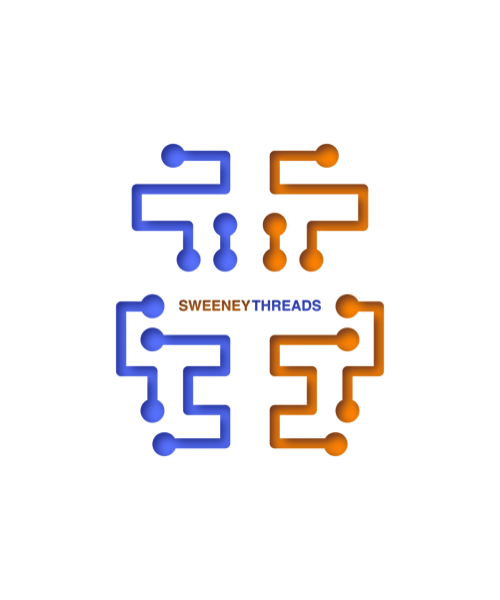
\includegraphics[scale=0.8]{sweeney.png}
		\end{figure}
		\begin{center}
			Versione 0.1.0
		\end{center}
		% Date, change the \today to a set date if you want to be precise
		{\large \today}\\[3cm] 
		% Fill the rest of the page with whitespace
		\vfill  
	\end{titlepage}
	
	
	\tableofcontents
	
	\newpage 
	\section*{Diario delle modifiche}
		\begin{table}[H]
			\begin{tabularx}{\textwidth}{s f m X}
				\noalign{\hrule height 1.5pt}
				\rowcolor{orange!85} Versione & Data & Autore & Descrizione \\
                \noalign{\hrule height 0.5pt}
				0.1.0 & 2016-04-10 & \emph{Progettista} \newline Nicoletti Luca & Sistemazione errori rilevati dalla verifica effettuata in versione 0.0.12 \\
				\noalign{\hrule height 0.5pt}
				0.0.12 & 2016-04-10 & \emph{Verificatore} \newline Bortolazzo Matteo & Verificato l'intero documento, segnalati vari errori in tutte le sezioni\\
				\noalign{\hrule height 0.5pt}
				0.0.11 & 2016-04-10 & \emph{Progettista} \newline Maino Elia & Completata la descrizione di classe e interfacce del componente server\\
				\noalign{\hrule height 0.5pt}
				0.0.10 & 2016-04-10 & \emph{Progettista} \newline Nicoletti Luca & Modificate e inserite le nuove immagini dei packages e delle classi per 
                la sezione Server (4.2). Modificate le immagini nei diagrammi di sequenza (Sezione 6) e modificate le descrizioni di tutti in modo da 
                uniformarle. Cambiate le immagini dei Design Pattern (Sezione 9.1)\\
				\noalign{\hrule height 0.5pt}
				0.0.9 & 2016-04-10 & \emph{Progettista} \newline Padovan Tommaso & Incremento sezione Componenti e Classi: allineata sezione Driver allo standard, stesura sezione Client. \\
				\noalign{\hrule height 0.5pt}
				0.0.8 & 2016-04-09 & \emph{Progettisti} \newline Bonato Paolo \newline Biggeri Mattia & Stesura sezione tracciamento componenti-requisiti.\\
                \noalign{\hrule height 0.5pt}
				0.0.7 & 2016-04-09 & \emph{Progettista} \newline Nicoletti Luca & Inseriti tutti i diagrammi di sequenza riguardanti l'implementazione 
                di richieste lato server, sostituita immagine dei Packages generale. Inserita una breve spiegazione di ogni diagramma di sequenza\\
				\noalign{\hrule height 0.5pt}
				0.0.6 & 2016-04-09 & \emph{Progettisti} \newline Biggeri Mattia \newline Padovan Tommaso \newline Bonato Paolo & Stesura sezioni 
                Driver, Diagrammi attività, Stime di fattibilità e bisogno di risorse;  aggiunta immagine nella sezione 3.2.3, aggiunto Singleton 
                nelle descrizioni dei Design Pattern, aggiornata leggenda.\\
				\noalign{\hrule height 0.5pt}
				0.0.5 & 2016-04-08 & \emph{Progettisti} \newline Maino Elia \newline Nicoletti Luca \newline Bortolazzo Matteo & Stesura sezione riguardante le componenti dell'architettura lato server: diagrammi dei package e delle classi e descrizioni testuali   \\
				\noalign{\hrule height 0.5pt}
				0.0.4 & 2016-04-06 & \emph{Progettisti} \newline Biggeri Mattia \newline Tommasin Davide & Aggiunta sezione 
                in appendice suoi Design Pattern, contiene al momento la descrizione di: MVC, Event-driven, Command   \\
				\noalign{\hrule height 0.5pt}
				0.0.3 & 2016-04-03 & \emph{Progettista} \newline Bonato Paolo & Accorpate le sezioni "Componenti", "Package" e "Classi" in "Componenti e classi". Riadattata la sezione "Metodo e formalismo di specifica" alla nuova struttura. Inserite le immagini 1 e 2. Apportate le correzioni indicate. \\
                \noalign{\hrule height 0.5pt}
				0.0.2 & 2016-03-26 & \emph{Progettisti} \newline Bonato Paolo \newline Biggeri Mattia \newline Padovan Tommaso 
                \newline Tommasin Davide \newline Bortolazzo Matteo & Prima stesura di Architettura generale (sezione 3) e componenti (sezione 4)\\
				\noalign{\hrule height 0.5pt}
				0.0.1 & 2016-03-24 & \emph{Analisti} \newline Bonato Paolo \newline Biggeri Mattia & Creazione scheletro documento, stesura introduzione, definizione di metodo e formalismo di specifica. \\
				\noalign{\hrule height 1.5pt}
			\end{tabularx}
			\caption{Diario delle modifiche \label{tab:table_label}}
		\end{table}
	



	\newpage \section{Introduzione}
	\subsection{Scopo del documento}
		Il documento definisce la progettazione ad alto livello del progetto Actorbase.
		Verrà presentata l'architettura generale, le componenti, le classi e i design pattern utilizzati per realizzare il prodotto.
	\subsection{Scopo del prodotto}
		Il progetto consiste nella realizzazione di un Database NoSQL key-value basato sul modello ad 
		Attori con l'obiettivo di fornire una tecnologia adatta allo sviluppo di moderne 
		applicazioni che richiedono brevissimi tempi di risposta e che elaborano enormi quantità 
		di dati. Lo sviluppo porterà al rilascio del software sotto licenza MIT.
	\subsection{Glossario}
		Al fine di evitare ambiguità di linguaggio e di massimizzare la comprensione dei documenti, il 
      gruppo ha steso un documento interno che è il \emph{Glossario v1.3.0}. In esso saranno definiti, in modo
      chiaro e conciso i termini che possono causare ambiguità o incomprensione del testo.
	\subsection{Riferimenti}
		\begin{itemize}
			\item \textbf{Slide dell'insegnamento Ingegneria del software mod.A:} \\
			\url{http://www.math.unipd.it/~tullio/IS-1/2015/Dispense/E02.pdf}
			\item \textbf{Scala:} \\
			\url{http://www.scala-lang.org/}
			\item \textbf{Java:} \\
			\url{http://www.java.com/}
			\item \textbf{Akka:} \\
			\url{http://akka.io/}
			\item \textbf{IntelliJ:} \\
			\url{http://www.jetbrains.com/idea/}
		\end{itemize}
	\subsubsection{Normativi}
		\begin{itemize}
			\item \textbf{Norme di progetto:} \emph{Norme di progetto v1.3.5}
			\item \textbf{Capitolato d'appalto Actorbase (C1):} \\ 
			\url{http://www.math.unipd.it/~tullio/IS-1/2015/Progetto/C1p.pdf}
		\end{itemize}
		
		
	\newpage 
	\section{Tecnologie utilizzate}
	\subsection{Scala}
		Le possibili scelte dettate dal capitolato sono Java e Scala. Si è scelto di utilizzare Scala perché offre i seguenti vantaggi:
		\begin{itemize}
            \item \textbf{Completamente Object-Oriented:} A differenza di Java, Scala è completamente orientato agli oggetti. Non c'è distinzione del tipo: oggetto - tipo primitivo, ogni valore è semplicemente un oggetto.
			\item \textbf{Staticamente tipato:} \'E un linguaggio tipato staticamente, questo permette di effettuare più facilmente i test. Inoltre Scala è in grado di stabilire il tipo di un oggetto per inferenza.
            \item \textbf{Può eseguire codice Java:} Scala può eseguire codice scritto in Java. \'E dunque possibile utilizzare classi e librerie scritte in Java all'interno di programmi scritti in Scala. 
            \item \textbf{Concorrenza e distribuzione:} Ottimo supporto alla programmazione multi-threaded e distribuita, essenziale per la realizzazione di un prodotto responsive e scalabile.
			\item \textbf{Supporto alla definizione di DSL:} Scala supporta nativamente la definizione di DSL.
            \item \textbf{Supporto di Akka:} Il linguaggio supporta la libreria Akka che è richiesta dal capitolato.
		\end{itemize}
		Inoltre il Committente ha espresso esplicitamente la sua preferenza sull'utilizzo di Scala.
		\begin{figure} [H]
			\centering
			
\includegraphics[scale=0.15]{immagini/ST/scala.png}
			\caption{Scala - logo}
		\end{figure}	
	\subsection{Akka}
		L'utilizzo della libreria Akka oltre ad essere reso obbligatorio dal committente, fornisce un'eccellente base su cui sviluppare un sistema basato sul modello ad attori.
        Akka permette di costruire facilmente applicazioni message-driven che siano estremamente concorrenti, distribuite e resilienti.         
        La natura distribuita e asincrona degli attori messi a disposizione da Akka soddisfa pienamente i bisogni del sistema da implementare.
	\begin{figure} [H]
			\centering
			
\includegraphics[scale=0.45]{immagini/ST/Akka.png}
			\caption{Akka - logo}
		\end{figure}	
	
	
	\newpage 
	\section{Descrizione dell'architettura}
		\subsection{Metodo e formalismo di specifica}
			Nell'esposizione dell'architettura del prodotto si procederà con un approccio di tipo top-down, ovvero dal generale al particolare. \\
			Inizialmente si descriveranno le tre componenti fondamentali: Client, Server e Driver; poi le componenti più piccole al loro interno, specificando i package e le classi che li compongono. \\ \\
			Per ogni package saranno descritti brevemente il tipo, l'obiettivo e la funzione e saranno specificati eventuali figli, classi ed interazioni con altri package.
			Ogni classe sarà dotata di una breve descrizione e ne saranno specificate le responsabilità, le classi ereditate, le sottoclassi e le relazioni con altre classi. \\
			Successivamente saranno mostrati e descritti i diagrammi delle attività che coinvolgono l'utente. \\
			Infine si illustreranno degli esempi di utilizzo dei design pattern nell'architettura del sistema.
		\subsection{Architettura generale}
        	L'architettura generale del sistema è di tipo client-server. \\ \\
            Il server ha un'architettura di tipo event-driven basata sul modello ad attori ed espone delle API tramite socket TCP. \\ \\
            L'architettura del Client segue il design pattern Model-View-Controller con interfaccia da linea di comando e comunica con il server  grazie ad un driver tramite connessione TCP.
            
        \begin{figure} [H]
			\centering
			\includegraphics[scale=0.25]{Packages_Generale.png}
			\caption{Architettura generale, vista Package}
		\end{figure}
		
		\begin{figure} [H]
			\centering
			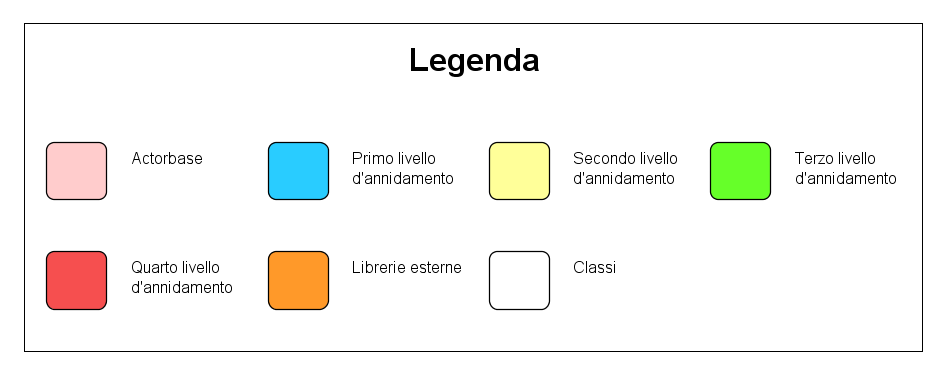
\includegraphics[scale=0.3]{ST/Legenda.png}
			\caption{Legenda}
		\end{figure}
            \subsubsection{Server}
        	Il server di \emph{Actorbase} è composto da due package principali: il package \textbf{Core} e il package \textbf{API}. \\
            Il package \textbf{Core} è a sua volta composto dal package \textbf{Actors}, contenente le classi che definiscono gli attori del sistema, e dal package \textbf{messages}, contenente i messaggi che gli attori possono inviarsi tra loro. \\
            Il package \textbf{API} contiene le classi che forniscono una comunicazione con i client esterni.
            \begin{figure} [H]
			\centering
			\includegraphics[scale=0.35]{Server/Package/serverALL.png}
			\caption{Server, vista Package}
		\end{figure}
        \subsubsection{Client}
        	L'architettura del Client seguirà il design pattern MVC:
            \begin{itemize}
				\item \textbf{Model:}
                	Il Model è la componente che si occupa di comunicare con il server usando i metodi del driver e di notificare la View quando avviene un cambiamento nel suo stato.
                \item \textbf{View:}
                	La View è la componente che interagisce con l'utente mediante interfaccia a linea di comando. L'utente può usare il DSL per interrogare il Model. La View esegue delle \emph{state query} sul model per avere le informazioni aggiornate.
                \item \textbf{Controller:}
                	Il Controller è la componente che esegue il parsing dei comandi del DSL inseriti nella View e li notifica al Model.			
			\end{itemize}
        
        \subsubsection{Driver}
        	Il Driver è una libreria, invocando i metodi della quale è possibile effettuare richieste TCP verso le API esposte dal Server.
        \begin{figure} [H]
			\centering
			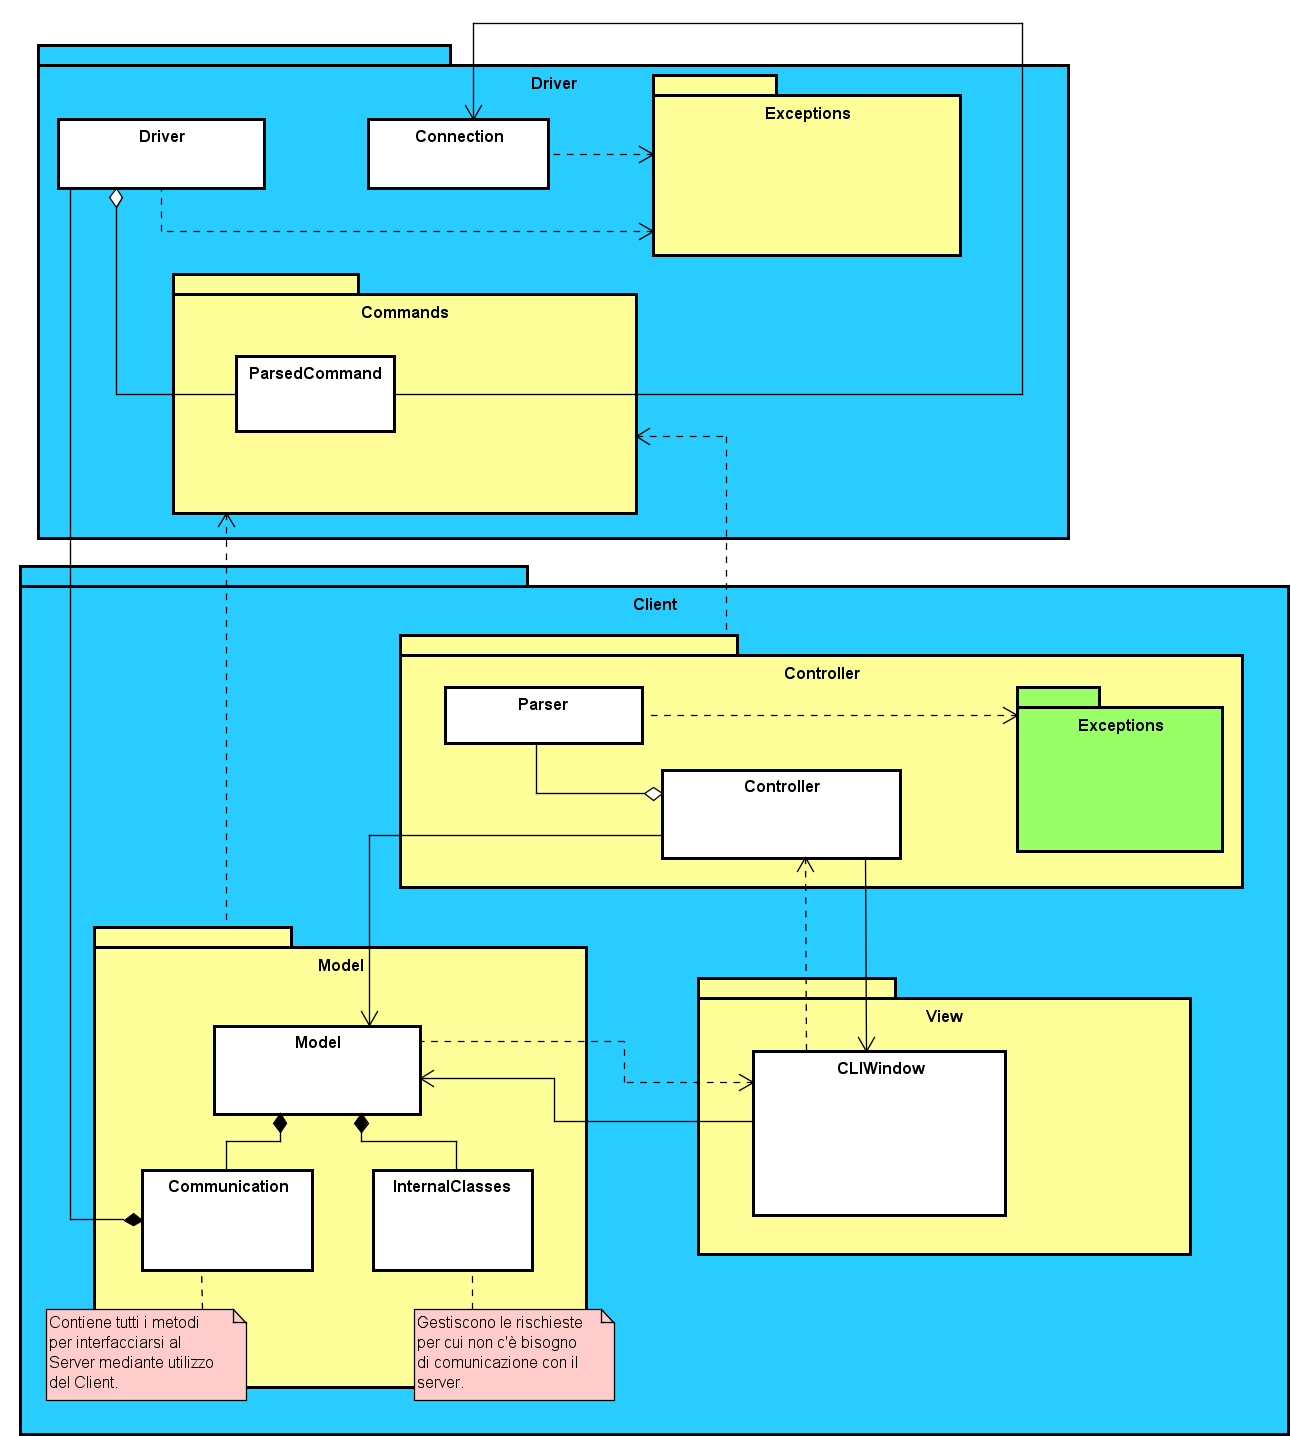
\includegraphics[scale=0.35]{ST/Client/GeneraleClient.png}
        	\caption{Architettura generale Client e Driver}
		\end{figure}
            
	\newpage 
	\section{Componenti e Classi}
		\subsection{Actorbase}
			\begin{figure} [H]
			\centering
			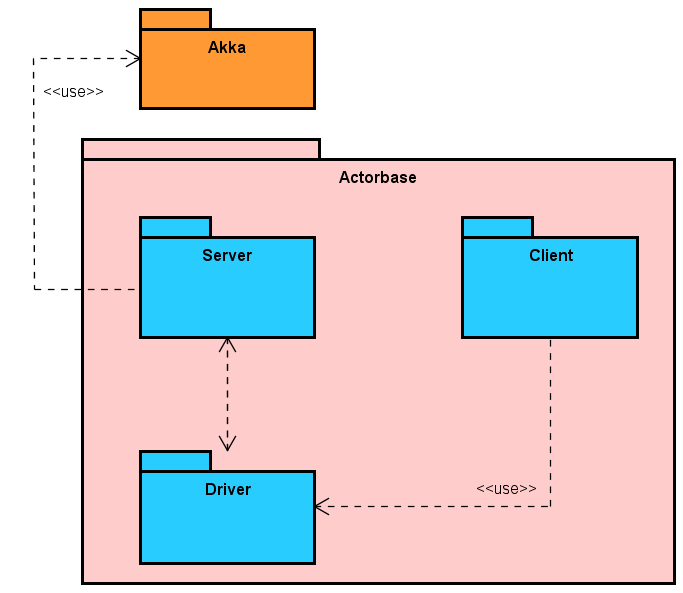
\includegraphics[scale=0.50]{Server/Package/actorbase.png}
			\caption{Componente Actorbase}
		\end{figure}
			\subsubsection{Descrizione}
				È il package principale del sistema. L'interazione tra i package \textbf{Server} e \textbf{Driver} definiscono una comunicazione su rete di tipo client-server. \\ Le classi definite nel package \textbf{Server} utilizzano ed estendono le classi della libreria Akka.
			\subsubsection{Package Figli}
				\begin{itemize}
					\item Actorbase.Server
					\item Actorbase.Client
					\item Actorbase.Driver
					\item Actorbase.Akka
				\end{itemize}
		\subsection{Actorbase.Server}
			\begin{figure}[H]
			\centering
			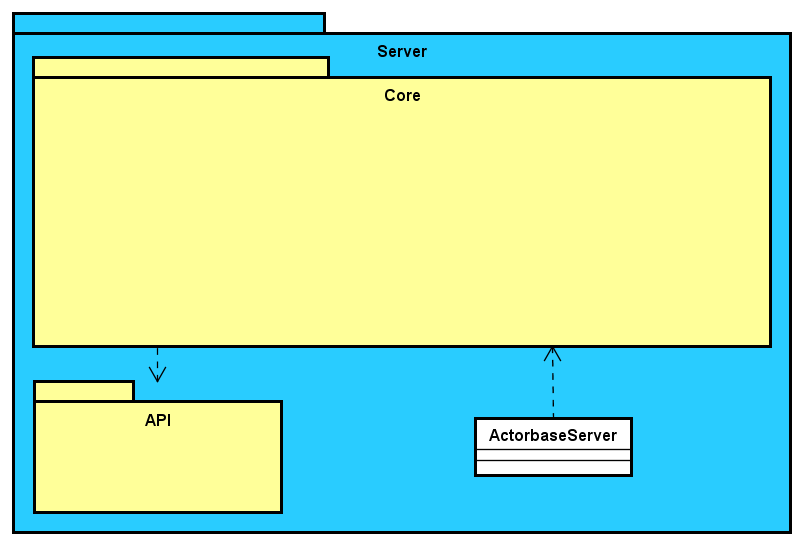
\includegraphics[scale=0.50]{Server/Package/ServerLevel.png}
			\caption{Componente Actorbase.Server}
			\end{figure}
			\subsubsection{Descrizione}
				Package per la componente lato server del sistema. È composto dai packages \textbf{Core} ed \textbf{API} e dalla classe \emph{ActorbaseServer}.
			\subsubsection{Package Figli}
				\begin{itemize}
					\item Actorbase.Server.Core
					\item Actorbase.Server.API
				\end{itemize}
			\subsubsection{Classi}
			\begin{itemize}
				\item Actorbase.Server.ActorbaseServer
			\end{itemize}
		\subsection{Actorbase.Server.API}
			\begin{figure} [H]
			\centering
			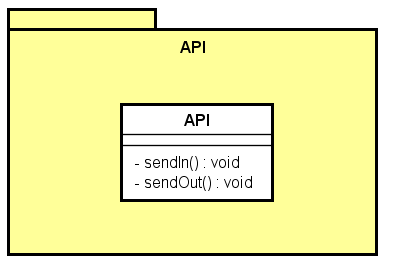
\includegraphics[scale=0.70]{Server/Package/APILevel.png}
			\caption{Componente Actorbase.Server.API}
			\end{figure}
			\subsubsection{Descrizione}
				Package contenenti le classi che definiscono le API attraverso cui i client possono interfacciarsi all'istanza di un server del sistema.
			\subsubsection{Classi}
			\begin{itemize}
				\item Actorbase.Server.API.API
			\end{itemize}
			
			\subsection{Actorbase.Server.API.API}
			\subsubsection{Descrizione}
				Classe \emph{singleton} che definisce l'insieme di API esposte dal server e il loro utilizzo.
			\subsubsection{Utilizzo}
				Viene utilizzata per gestire l'insieme di connessioni del server dall'esterno, e per accettarne di nuove. Inoltra le richieste provenienti dall'esterno all'actor Main e invia le risposte ai client.
			\subsubsection{Relazione con altre classi}
			\begin{itemize}
				\item \textbf{Actorbase.Server.Core.Actors.Storefinder.Main} 
			\end{itemize}
			
		\subsection{Actorbase.Server.Core}
			\begin{figure} [H]
			\centering
			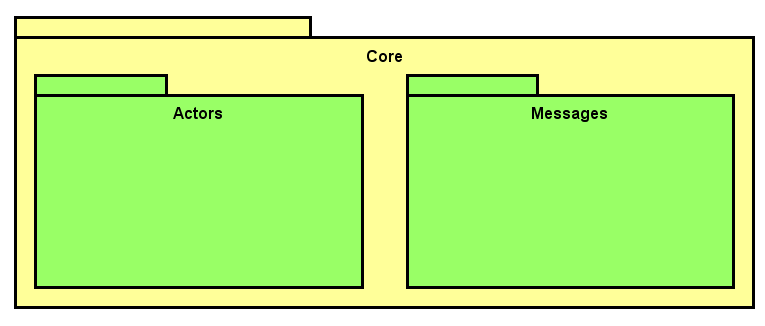
\includegraphics[scale=0.55]{Server/Package/CoreLevel.png}
			\caption{Componente Actorbase.Server.Core}
			\end{figure}
			\subsubsection{Descrizione}
				Il package contiene le componenti che costituiscono il nucleo del sistema logico lato server. \'E composto da due package: \textbf{Actors} e \textbf{Messages}
			\subsubsection{Package figli}
			\begin{itemize}
				\item Actorbase.Server.Core.Actors
				\item Actorbase.Server.Core.Messages
			\end{itemize}
			
		\subsection{Actorbase.Server.Core.Actors}
			\begin{figure} [H]
			\centering
			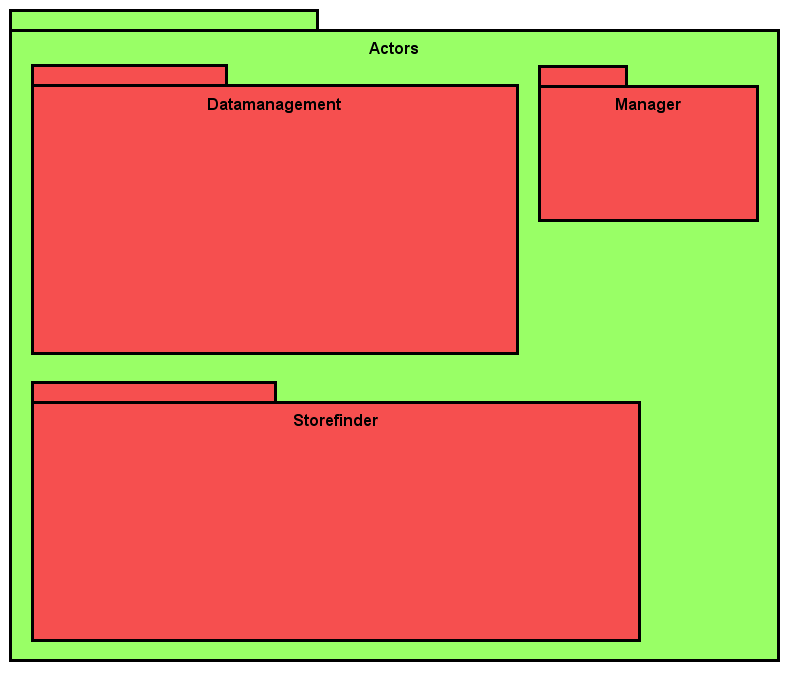
\includegraphics[scale=0.50]{Server/Package/ActorsLevel.png}
			\caption{Componente Actorbase.Server.Core.Actors}
			\end{figure}
			\subsubsection{Descrizione}
				Il package contiene le componenti che costituiscono i diversi attori definiti nel sistema. Essi definiscono le diverse categorie di attori.
			\subsubsection{Package figli}
			\begin{itemize}
				\item Actorbase.Server.Core.Actors.Datamanagement
				\item Actorbase.Server.Core.Actors.Manager
				\item Actorbase.Server.Core.Actors.Storefinder
			\end{itemize}
			
			\subsection{Actorbase.Server.Core.Actors.Datamanagement}
			\begin{figure} [H]
			\centering
			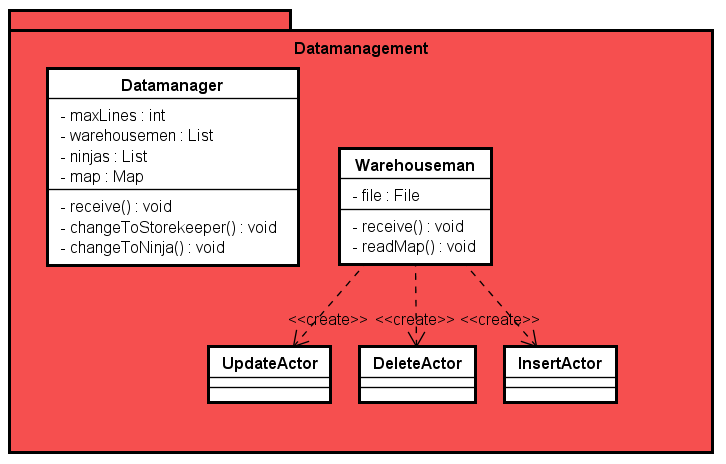
\includegraphics[scale=0.55]{Server/Package/DatamanagementLevel.png}
			\caption{Componente Actorbase.Server.Core.Actors.Datamanagement}
			\end{figure}
			\subsubsection{Descrizione}
				All'interno di questo package sono definite le classi che rappresentano gli attori che si occupano direttamente della gestione dei dati.
			\subsubsection{Classi}
			\begin{itemize}
				\item Actorbase.Server.Core.Actors.Datamanagement.Datamanager
				\item Actorbase.Server.Core.Actors.Datamanagement.Warehouseman
				\item Actorbase.Server.Core.Actors.Datamanagement.UpdateActor
				\item Actorbase.Server.Core.Actors.Datamanagement.DeleteActor
				\item Actorbase.Server.Core.Actors.Datamanagement.InsertActor
			\end{itemize}
			
		\subsection{Actorbase.Server.Core.Actors.Datamanagement.Datamanager}
			\subsubsection{Descrizione}
				Classe che definisce un actor di tipo Datamanager.
			\subsubsection{Utilizzo}
				Si utilizza per mantenere in RAM una porzione di una mappa di un Database. Un oggetto Datamanager possiede due comportamenti diversi: uno nel caso funzioni da copia principale dei dati (Storekeeper) e l'altro nel caso funzioni da copia di backup (Ninja).
			\subsubsection{Relazioni con altre classi}
				Nessuna.
			
		\subsection{Actorbase.Server.Core.Actors.Datamanagement.Warehouseman}
			\subsubsection{Descrizione}
				Classe che definisce un actor di tipo Warehouseman.
			\subsubsection{Utilizzo}
				Si utilizza per mantenere persistenza su disco di una porzione di una mappa di un Database.
			\subsubsection{Relazioni con altre classi}
			\begin{itemize}
				\item Actorbase.Server.Core.Actors.Datamanagement.UpdateActor
				\item Actorbase.Server.Core.Actors.Datamanagement.DeleteActor
				\item Actorbase.Server.Core.Actors.Datamanagement.InsertActor
			\end{itemize}
			
		\subsection{Actorbase.Server.Core.Actors.Datamanagement.UpdateActor}
			\subsubsection{Descrizione}
				Classe che definisce un actor di tipo UpdateActor.
			\subsubsection{Utilizzo}
				Si utilizza per aggiornare un item su un file su disco.
			\subsubsection{Relazioni con altre classi}
				Nessuna.
			
		\subsection{Actorbase.Server.Core.Actors.Datamanagement.DeleteActor}
			\subsubsection{Descrizione}
				Classe che definisce un actor di tipo DeleteActor.
			\subsubsection{Utilizzo}
				Si utilizza per rimuovere un item su un file su disco. 
			\subsubsection{Relazioni con altre classi}
				Nessuna.
			
		\subsection{Actorbase.Server.Core.Actors.Datamanagement.InsertActor}
			\subsubsection{Descrizione}
				Classe che definisce un actor di tipo InsertActor.
			\subsubsection{Utilizzo}
				Si utilizza per inserire un item su un file su disco. 
			\subsubsection{Relazioni con altre classi}
				Nessuna.

		\subsection{Actorbase.Server.Core.Actors.Manager}
			\begin{figure} [H]
			\centering
			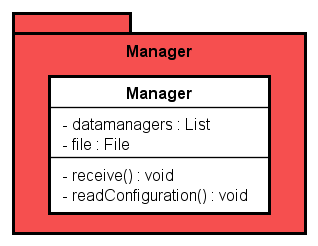
\includegraphics[scale=0.65]{Server/Package/ManagerLevel.png}
			\caption{Componente Actorbase.Server.Core.Actors.Manager}
			\end{figure}
			\subsubsection{Descrizione}
				All'interno di questo package sono definite le classi che rappresentano gli attori che si occupano della gestione di altri attori e dei vincoli presenti su di essi.
			\subsubsection{Classi}
			\begin{itemize}
				\item Actorbase.Server.Core.Actors.Manager.Manager
			\end{itemize}
			
		\subsection{Actorbase.Server.Core.Actors.Manager.Manager}
			\subsubsection{Descrizione}
				Classe che definisce un actor di tipo Manager.
			\subsubsection{Utilizzo}
				Un oggetto di tipo Manager è utilizzato per gestire vincoli su altri attori.
			\subsubsection{Relazioni con altre classi}
			\begin{itemize}
				\item Actorbase.Server.Core.Actors.Datamanagement.Datamanager
			\end{itemize}
			
		\subsection{Actorbase.Server.Core.Actors.Storefinder}
			\begin{figure} [H]
			\centering
			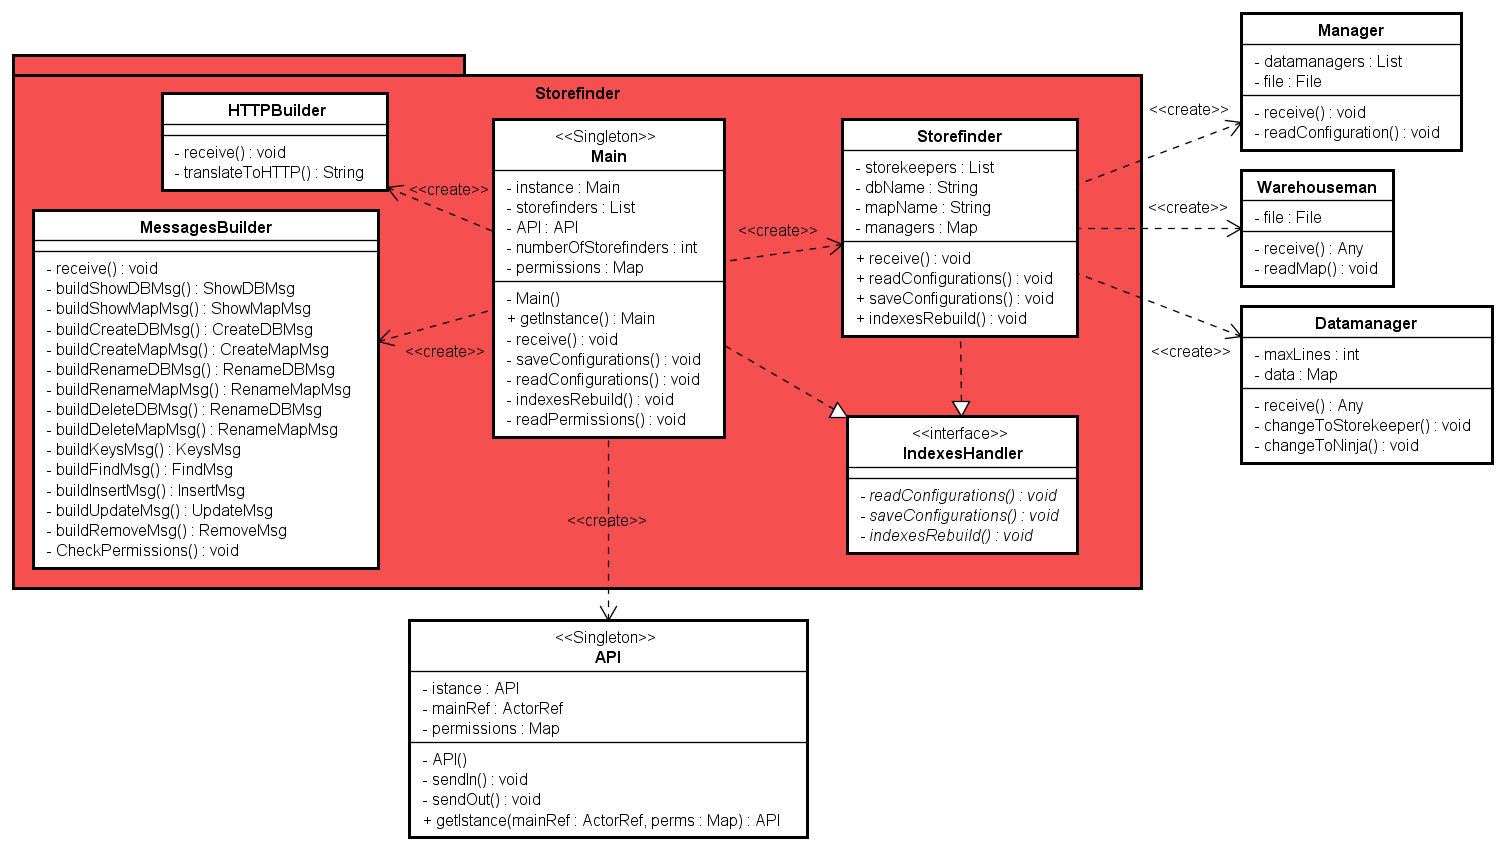
\includegraphics[width=\textwidth]{Server/Package/StorefinderLevel.png}
			\caption{Componente Actorbase.Server.Core.Actors.Storefinder}
			\end{figure}
			\subsubsection{Descrizione}
				All'interno di questo package sono definite le classi che rappresentano gli attori che si occupano dell'indicizzazione degli altri attori presenti e del corretto instradamento, creazione e gestione dei messaggi.
			\subsubsection{Classi}
			\begin{itemize}
				\item Actorbase.Server.Core.Actors.Storefinder.Storefinder
				\item Actorbase.Server.Core.Actors.Storefinder.Main
				\item Actorbase.Server.Core.Actors.Storefinder.HTTPBuilder
				\item Actorbase.Server.Core.Actors.Storefinder.MessagesBuilder
			\end{itemize}
			\subsubsection{Interfacce}
			\begin{itemize}
				\item Actorbase.Server.Core.Actors.Storefinder.IndexesHandler
			\end{itemize}

		\subsection{Actorbase.Server.Core.Actors.Storefinder.IndexesHandler}
			\subsubsection{Descrizione}
				Interfaccia per gli attori che si occupano di indicizzare altri attori e di inviare messaggi e ricevere risposte da essi. Definisce i contratti di metodi che permettono di leggere, salvare e ricostruire un insieme di indici.
			\subsubsection{Classi figlie}
			\begin{itemize}
				\item Actorbase.Server.Core.Actors.Storefinder.Main
				\item Actorbase.Server.Core.Actors.Storefinder.Storefinder
			\end{itemize}

		\subsection{Actorbase.Server.Core.Actors.Storefinder.Storefinder}
			\subsubsection{Descrizione}
				Classe che definisce un actor di tipo Storefinder. Implementa l'interfaccia IndexesHandler.
			\subsubsection{Utilizzo}
				Uno Storefinder indicizza un insieme di Datamanager rappresentanti diverse porzioni di una stessa mappa. Per ogni Datamanager indicizzato, inoltre, tiene traccia dei Datamanager Ninja e dei Warehouseman ad esso associati. Si occupa di inviare gli opportuni messaggi a tali tipologie di attori, di ricevere e instradare le risposte ricevute. 
				\\ Uno Storefinder inoltre si occupa della creazione e distruzione di attori di tipo Manager, Datamanager, Warehouseman.
			\subsubsection{Relazioni con altre classi}
			\begin{itemize}
				\item \textbf{Actorbase.Server.Core.Actors.Storefinder.Main:} relazione entrante, creazione
				\item \textbf{Actorbase.Server.Core.Actors.Manager.Manager:} relazione uscente, creazione
				\item \textbf{Actorbase.Server.Core.Actors.Datamanagement.Datamanager:} relazione uscente, creazione
				\item \textbf{Actorbase.Server.Core.Actors.Datamanagement.Warehouseman:} relazione uscente, creazione
			\end{itemize}
			\subsubsection{Interfacce implementate}
			\begin{itemize}
				\item \textbf{Actorbase.Server.Core.Actors.Storefinder.IndexesHandler} 
			\end{itemize}

		\subsection{Actorbase.Server.Core.Actors.Storefinder.Main}
			\subsubsection{Descrizione}
				Classe \emph{singleton} che definisce un actor di tipo Main. Implementa l'interfaccia IndexesHandler.
			\subsubsection{Utilizzo}
				Il Main indicizza un insieme di Storefinder e con essi scambia messaggi, inoltre si occupa di inviare e ricevere messaggi HTTP da API. Crea attori di tipo Storefinder, MessagesBuilder, HTTPBuilder.
			\subsubsection{Relazioni con altre classi}
			\begin{itemize}
				\item \textbf{Actorbase.Server.ActorbaseServer:} relazione entrante, creazione
				\item \textbf{Actorbase.Server.Core.Actors.Storefinder.Storefinder:} relazione uscente, creazione
				\item \textbf{Actorbase.Server.Core.Actors.Storefinder.MessagesBuilder:} relazione uscente, creazione
				\item \textbf{Actorbase.Server.Core.Actors.Storefinder.HTTPBuilder:} relazione uscente, creazione
				\item \textbf{Actorbase.Server.Core.Actors.API.API:} relazione uscente, creazione
			\end{itemize}
			\subsubsection{Interfacce implementate}
			\begin{itemize}
				\item \textbf{Actorbase.Server.Core.Actors.Storefinder.IndexesHandler} 
			\end{itemize}

		\subsection{Actorbase.Server.Core.Actors.Storefinder.MessagesBuilder}
			\subsubsection{Descrizione}
				Classe che definisce un actor di tipo MessagesBuilder.
			\subsubsection{Utilizzo}
				Costruisce uno dei messaggi definiti in \textbf{Actorbase.Server.Core.Messages} a partire da un messaggio HTTP, basandosi sui permessi del client che ha inviato il messaggio HTTP.
			\subsubsection{Relazioni con altre classi}
			\begin{itemize}
				\item \textbf{Actorbase.Server.Core.Actors.Storefinder.Main:} relazione entrante, creazione
			\end{itemize}

		\subsection{Actorbase.Server.Core.Actors.Storefinder.HTTPBuilder}
			\subsubsection{Descrizione}
				Classe che definisce un actor di tipo HTTPBuilder.
			\subsubsection{Utilizzo}
				Costruisce un messaggio HTTP che le API possono inviare a un client a partire da un messaggio definito in \textbf{Actorbase.Server.Core.Messages}.
			\subsubsection{Relazioni con altre classi}
			\begin{itemize}
				\item \textbf{Actorbase.Server.Core.Actors.Storefinder.Main:} relazione entrante, creazione
			\end{itemize}
		
		\subsection{Actorbase.Server.Core.Messages}
			\begin{figure} [H]
			\centering
			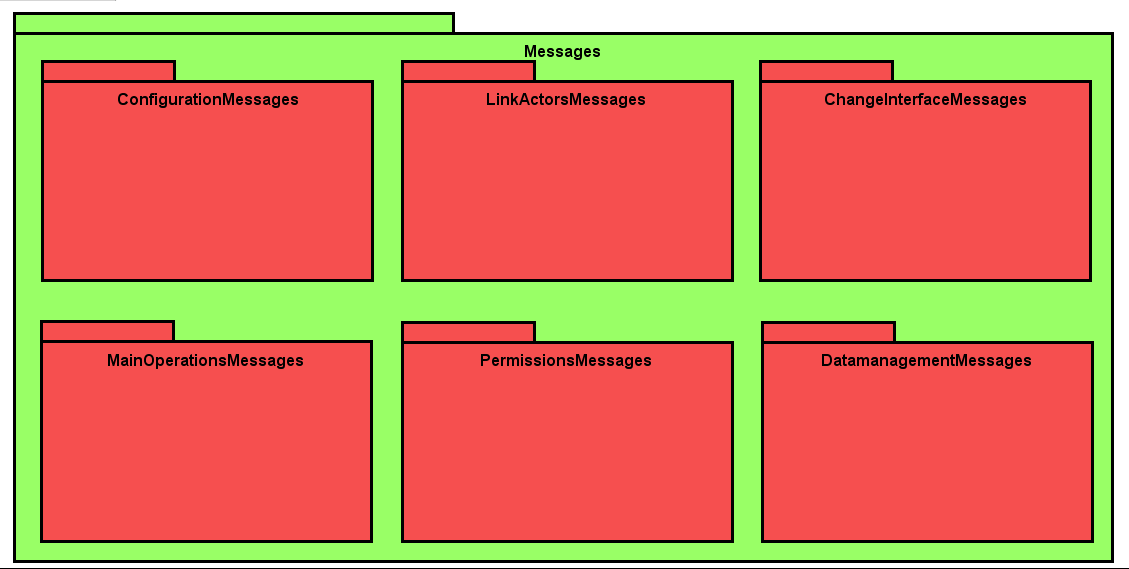
\includegraphics[scale=0.55]{Server/Package/MessagesLevel.png}
			\caption{Componente Actorbase.Server.Core.Messages}
			\end{figure}
			\subsubsection{Descrizione}
				All'interno di questo package sono definite le componenti che rappresentano i messaggi che i diversi attori del sistema possono inviarsi tra loro.
			\subsubsection{Package Figli}
			\begin{itemize}
				\item Actorbase.Server.Core.Messages.ConfigurationMessages
				\item Actorbase.Server.Core.Messages.PermissionMessages
				\item Actorbase.Server.Core.Messages.LinkActorsMessages
				\item Actorbase.Server.Core.Messages.MainOperationMessages
				\item Actorbase.Server.Core.Messages.DatamanagementMessages
				\item Actorbase.Server.Core.Messages.ChangeInterfaceMessages
			\end{itemize}
			
			\subsection{Actorbase.Server.Core.Messages.ConfigurationMessages}
			\begin{figure} [H]
			\centering
			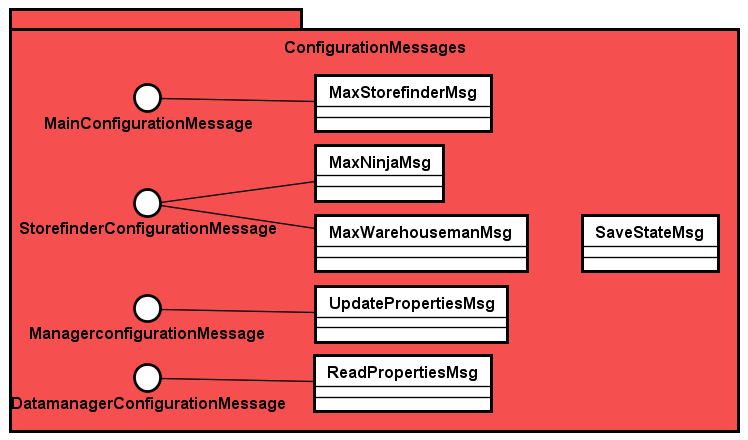
\includegraphics[scale=0.55]{Server/Package/ConfigurationMessagesLevel.png}
			\caption{Componente Actorbase.Server.Core.Messages.ConfigurationMessages}
			\end{figure}
			\subsubsection{Descrizione}
				All'interno di questo package sono definite le classi e le interfacce che rappresentano i messaggi relativi ad avvisi di configurazione delle impostazioni del sistema.
			\subsubsection{Classi}
			\begin{itemize}
				\item Actorbase.Server.Core.Messages.ConfigurationMessages.MaxStorefinderMsg
				\item Actorbase.Server.Core.Messages.ConfigurationMessages.MaxNinjaMsg
				\item Actorbase.Server.Core.Messages.ConfigurationMessages.MaxWarehousemanMsg
				\item Actorbase.Server.Core.Messages.ConfigurationMessages.UpdatePropertiesMsg
				\item Actorbase.Server.Core.Messages.ConfigurationMessages.ReadPropertiesMsg
				\item Actorbase.Server.Core.Messages.ConfigurationMessages.SaveStateMsg
			\end{itemize}
			\subsubsection{Interfacce}
			\begin{itemize}
				\item Actorbase.Server.Core.Messages.ConfigurationMessages.MainConfigurationMessage
				\item Actorbase.Server.Core.Messages.ConfigurationMessages.StorefinderConfigurationMessage
				\item Actorbase.Server.Core.Messages.ConfigurationMessages.ManagerConfigurationMessage
				\item Actorbase.Server.Core.Messages.ConfigurationMessages.DatamanagerConfigurationMessage
			\end{itemize}

			\subsection{Actorbase.Server.Core.Messages.ConfigurationMessages.\\ MainConfigurationMessage}
			\subsubsection{Descrizione}
				Interfaccia per messaggi di configurazione per actor di tipo Main. 
				Le classi che implementano questa interfaccia definiscono messaggi di configurazione che possono essere gestiti da actor di tipo Main.
			\subsubsection{Classi figlie}
			\begin{itemize}
				\item Actorbase.Server.Core.Messages.ConfigurationMessages.MaxStorefinderMsg
			\end{itemize}

			\subsection{Actorbase.Server.Core.Messages.ConfigurationMessages.MaxStorefinderMsg}
			\subsubsection{Descrizione}
				Classe che definisce un messaggio MaxStorefinder.
			\subsubsection{Utilizzo}
				Un messaggio MaxStorefinder informa chi lo riceve di aggiornare l'impostazione relativa al numero di actor di tipo Storefinder creabili per mappa.
			\subsubsection{Relazioni con altre classi}
			\begin{itemize}
				\item \textbf{Actorbase.Server.ActorbaseServer:} relazione entrante, creazione
			\end{itemize}
			\subsubsection{Interfacce implementate}
			\begin{itemize}
				\item Actorbase.Server.Core.Messages.ConfigurationMessages.MainConfigurationMessage
			\end{itemize}

			\subsection{Actorbase.Server.Core.Messages.ConfigurationMessages.\\ StorefinderConfigurationMessage}
			\subsubsection{Descrizione}
				Interfaccia per messaggi di configurazione per actor di tipo Storefinder. 
				Le classi che implementano questa interfaccia definiscono messaggi di configurazione che possono essere gestiti da actor di tipo Storefinder.
			\subsubsection{Classi figlie}
			\begin{itemize}
				\item Actorbase.Server.Core.Messages.ConfigurationMessages.MaxNinjaMsg
				\item Actorbase.Server.Core.Messages.ConfigurationMessages.MaxWarehousemanMsg
			\end{itemize}

			\subsection{Actorbase.Server.Core.Messages.ConfigurationMessages.MaxNinjaMsg}
			\subsubsection{Descrizione}
				Classe che definisce un messaggio MaxNinjaMsg.
			\subsubsection{Utilizzo}
				Un messaggio MaxNinjaMsg informa chi lo riceve di aggiornare l'impostazione relativa al numero di actor di tipo Ninja creabili per Datamanager.
			\subsubsection{Relazioni con altre classi}
			\begin{itemize}
				\item \textbf{Actorbase.Server.ActorbaseServer:} relazione entrante, creazione
			\end{itemize}
			\subsubsection{Interfacce implementate}
			\begin{itemize}
				\item Actorbase.Server.Core.Messages.ConfigurationMessages.StorefinderConfigurationMessage
			\end{itemize}

			\subsection{Actorbase.Server.Core.Messages.ConfigurationMessages.MaxWarehousemanMsg}
			\subsubsection{Descrizione}
				Classe che definisce un messaggio MaxWarehousemanMsg.
			\subsubsection{Utilizzo}
				Un messaggio MaxWarehousemanMsg informa chi lo riceve di aggiornare l'impostazione relativa al numero di actor di tipo Warehouseman creabili per Datamanager.
			\subsubsection{Relazioni con altre classi}
			\begin{itemize}
				\item \textbf{Actorbase.Server.ActorbaseServer:} relazione entrante, creazione
			\end{itemize}
			\subsubsection{Interfacce implementate}
			\begin{itemize}
				\item Actorbase.Server.Core.Messages.ConfigurationMessages.StorefinderConfigurationMessage
			\end{itemize}

			\subsection{Actorbase.Server.Core.Messages.ConfigurationMessages.\\ ManagerConfigurationMessage}
			\subsubsection{Descrizione}
				Interfaccia per messaggi di configurazione per actor di tipo Manager. 
				Le classi che implementano questa interfaccia definiscono messaggi di configurazione che possono essere gestiti da actor di tipo Manager.
			\subsubsection{Classi figlie}
			\begin{itemize}
				\item Actorbase.Server.Core.Messages.ConfigurationMessages.UpdatePropertiesMsg
			\end{itemize}

			\subsection{Actorbase.Server.Core.Messages.ConfigurationMessages.UpdatePropertiesMsg}
			\subsubsection{Descrizione}
				Classe che definisce un messaggio UpdatePropertiesMsg.
			\subsubsection{Utilizzo}
				Un messaggio UpdatePropertiesMsg informa chi lo riceve di aggiornare le impostazioni per actor Manager.
			\subsubsection{Relazioni con altre classi}
			\begin{itemize}
				\item \textbf{Actorbase.Server.ActorbaseServer:} relazione entrante, creazione
			\end{itemize}
			\subsubsection{Interfacce implementate}
			\begin{itemize}
				\item Actorbase.Server.Core.Messages.ConfigurationMessages.ManagerConfigurationMessage
			\end{itemize}

			\subsection{Actorbase.Server.Core.Messages.ConfigurationMessages.\\ DatamanagerConfigurationMessage}
			\subsubsection{Descrizione}
				Interfaccia per messaggi di configurazione per actor di tipo Datamanager. 
				Le classi che implementano questa interfaccia definiscono messaggi di configurazione che possono essere gestiti da actor di tipo Datamanager.
			\subsubsection{Classi figlie}
			\begin{itemize}
				\item Actorbase.Server.Core.Messages.ConfigurationMessages.UpdatePropertiesMsg
			\end{itemize}

			\subsection{Actorbase.Server.Core.Messages.ConfigurationMessages.ReadPropertiesMsg}
			\subsubsection{Descrizione}
				Classe che definisce un messaggio ReadPropertiesMsg.
			\subsubsection{Utilizzo}
				Un messaggio ReadPropertiesMsg informa chi lo riceve di aggiornare le impostazioni per actor Datamanager.
			\subsubsection{Relazioni con altre classi}
			\begin{itemize}
				\item \textbf{Actorbase.Server.ActorbaseServer:} relazione entrante, creazione
			\end{itemize}
			\subsubsection{Interfacce implementate}
			\begin{itemize}
				\item Actorbase.Server.Core.Messages.ConfigurationMessages.DatamanagerConfigurationMessage
			\end{itemize}
			
			\subsection{Actorbase.Server.Core.Messages.PermissionMessages}
			\begin{figure} [H]
			\centering
			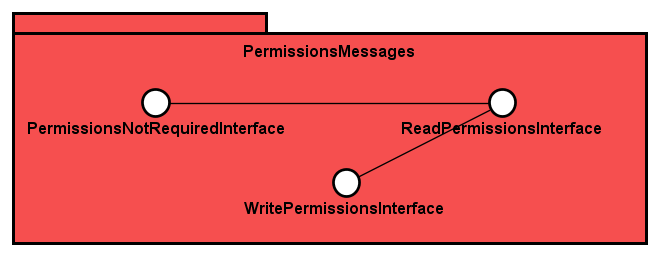
\includegraphics[scale=0.65]{Server/Package/PermissionsMessagesLevel.png}
			\caption{Componente Actorbase.Server.Core.Messages.PermissionMessages}
			\end{figure}
			\subsubsection{Descrizione}
				All'interno di questo package sono definite le interfacce che rappresentano i diversi gradi di permesso che un'operazione richiede. Un'operazione può infatti richiedere i permessi di lettura, scrittura o nessun permesso. Ogni messaggio relativo ad un'operazione richiesta da un client estende una di queste interfacce.
			\subsubsection{Interfacce}
			\begin{itemize}
				\item Actorbase.Server.Core.Messages.PermissionMessages.PermissionsNotRequiredInterface
				\item Actorbase.Server.Core.Messages.PermissionMessages.ReadPermissionsInterface
				\item Actorbase.Server.Core.Messages.PermissionMessages.WritePermissionsInterface
			\end{itemize}

			\subsection{Actorbase.Server.Core.Messages.PermissionMessages.\\ PermissionsNotRequiredInterface}
			\subsubsection{Descrizione}
				Interfaccia per messaggi che definiscono operazioni per le quali non sono richiesti specifici permessi.
			\subsubsection{Classi figlie}
			\begin{itemize}
				\item Actorbase.Server.Core.Messages.MainOperationMessage.ShowDBMsg
				\item Actorbase.Server.Core.Messages.MainOperationMessage.ShowMapMsg
				\item Actorbase.Server.Core.Messages.MainOperationMessage.CreateDBMsg
			\end{itemize}
			\subsubsection{Interfacce figlie}
			\begin{itemize}
				\item Actorbase.Server.Core.Messages.PermissionMessages.ReadPermissionsInterface
			\end{itemize}

			\subsection{Actorbase.Server.Core.Messages.PermissionMessages.ReadPermissionsInterface}
			\subsubsection{Descrizione}
				Interfaccia per messaggi che definiscono operazioni per le quali sono richiesti permessi di lettura.
			\subsubsection{Classi figlie}
			\begin{itemize}
				\item Actorbase.Server.Core.Messages.DatamanagementMessage.KeysMsg
				\item Actorbase.Server.Core.Messages.DatamanagementMessage.FindMsg
			\end{itemize}
			\subsubsection{Interfacce figlie}
			\begin{itemize}
				\item Actorbase.Server.Core.Messages.PermissionMessages.WritePermissionsInterface
			\end{itemize}
			\subsubsection{Interfacce estese}
			\begin{itemize}
				\item Actorbase.Server.Core.Messages.PermissionMessages.PermissionsNotRequiredInterface
			\end{itemize}

			\subsection{Actorbase.Server.Core.Messages.PermissionMessages.WritePermissionsInterface}
			\subsubsection{Descrizione}
				Interfaccia per messaggi che definiscono operazioni per le quali sono richiesti permessi di scrittura.
			\subsubsection{Classi figlie}
			\begin{itemize}
				\item Actorbase.Server.Core.Messages.MainOperationMessage.CreateMapMsg
				\item Actorbase.Server.Core.Messages.MainOperationMessage.RenameDBMsg
				\item Actorbase.Server.Core.Messages.MainOperationMessage.RenameMapMsg
				\item Actorbase.Server.Core.Messages.MainOperationMessage.DeleteDBMsg
				\item Actorbase.Server.Core.Messages.MainOperationMessage.DeleteMapMsg
				\item Actorbase.Server.Core.Messages.DatamanagementMessage.InsertMsg
				\item Actorbase.Server.Core.Messages.DatamanagementMessage.UpdateMsg
				\item Actorbase.Server.Core.Messages.DatamanagementMessage.RemoveMsg
			\end{itemize}
			\subsubsection{Interfacce estese}
			\begin{itemize}
				\item Actorbase.Server.Core.Messages.PermissionMessages.ReadPermissionsInterface
			\end{itemize}
			
			\subsection{Actorbase.Server.Core.Messages.LinkActorsMessages}
			\begin{figure} [H]
			\centering
			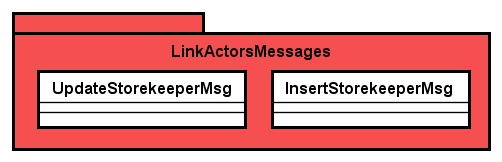
\includegraphics[scale=0.65]{Server/Package/LinkActorsMessagesLevel.png}
			\caption{Componente Actorbase.Server.Core.Messages.LinkActorsMessages}
			\end{figure}
			\subsubsection{Descrizione}
				All'interno di questo package sono definite le classi che rappresentano i messaggi relativi alla gestione dei collegamenti tra diversi attori.
			\subsubsection{Classi}
			\begin{itemize}
				\item Actorbase.Server.Core.Messages.LinkActorsMessages.UpdateStorekeeperMsg
				\item Actorbase.Server.Core.Messages.LinkActorsMessages.InsertStorekeeperMsg
			\end{itemize}

			\subsection{Actorbase.Server.Core.Messages.LinkActorsMessages.UpdateStorekeeperMsg}
			\subsubsection{Descrizione}
				Classe che definisce un messaggio UpdateStorekeeperMsg.
			\subsubsection{Utilizzo}
				Un messaggio UpdateStorekeeperMsg informa il Manager che lo riceve di aggiornare il riferimento ad uno degli actor Datamanager Storekeeper della sua lista.
			\subsubsection{Relazioni con altre classi}
			\begin{itemize}
				\item \textbf{Actorbase.Server.Core.Actors.Storefinder.Storefinder:} relazione entrante, creazione
			\end{itemize}

			\subsection{Actorbase.Server.Core.Messages.LinkActorsMessages.InsertStorekeeperMsg}
			\subsubsection{Descrizione}
				Classe che definisce un messaggio InsertStorekeeperMsg.
			\subsubsection{Utilizzo}
				Un messaggio InsertStorekeeperMsg informa il Manager che lo riceve di aggiungere il riferimento ad un actor Datamenager Storekeeper alla sua lista.
			\subsubsection{Relazioni con altre classi}
			\begin{itemize}
				\item \textbf{Actorbase.Server.Core.Actors.Storefinder.Storefinder:} relazione entrante, creazione
			\end{itemize}
			
			\subsection{Actorbase.Server.Core.Messages.MainOperationMessages}
			\begin{figure} [H]
			\centering
			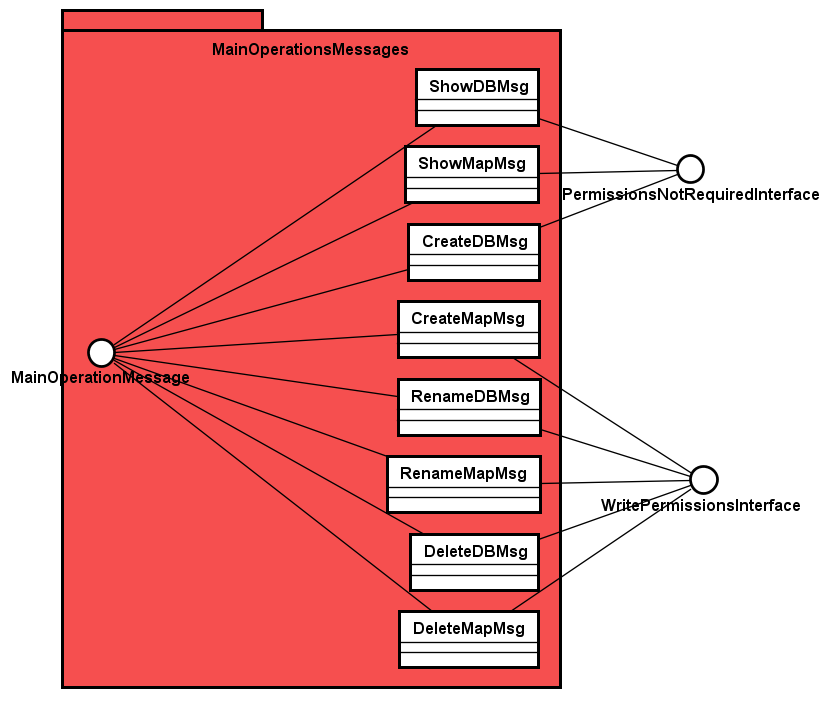
\includegraphics[scale=0.55]{Server/Package/MainOperationsMessagesLevel.png}
			\caption{Componente Actorbase.Server.Core.Messages.MainOperationMessages}
			\end{figure}
			\subsubsection{Descrizione}
				All'interno di questo package sono definite le classi e le interfacce che rappresentano i messaggi relativi ad operazioni che non richiedono l'inoltro del messaggio stesso.
			\subsubsection{Classi}
			\begin{itemize}
				\item Actorbase.Server.Core.Messages.MainOperationMessages.ShowDBMsg
				\item Actorbase.Server.Core.Messages.MainOperationMessages.ShowMapMsg
				\item Actorbase.Server.Core.Messages.MainOperationMessages.CreateDBMsg
				\item Actorbase.Server.Core.Messages.MainOperationMessages.CreateMapMsg
				\item Actorbase.Server.Core.Messages.MainOperationMessages.RenameDBMsg
				\item Actorbase.Server.Core.Messages.MainOperationMessages.RenameMapMsg
				\item Actorbase.Server.Core.Messages.MainOperationMessages.DeleteDBMsg
				\item Actorbase.Server.Core.Messages.MainOperationMessages.DeleteMapMsg
			\end{itemize}
			\subsubsection{Interfacce}
			\begin{itemize}
				\item Actorbase.Server.Core.Messages.MainOperationMessages.MainOperationMessage
			\end{itemize}

			\subsection{Actorbase.Server.Core.Messages.MainOperationMessages.ShowDBMsg}
			\subsubsection{Descrizione}
				Classe che definisce un messaggio ShowDBMsg.
			\subsubsection{Utilizzo}
				Un messaggio ShowDBMsg richiede la lista dei Database presenti sul server.
			\subsubsection{Relazioni con altre classi}
			\begin{itemize}
				\item \textbf{Actorbase.Server.Core.Actors.Storefinder.MessagesBuilder:} relazione entrante, creazione
			\end{itemize}
			\subsubsection{Interfacce estese}
			\begin{itemize}
				\item Actorbase.Server.Core.Messages.MainOperationMessages.MainOperationMessage
				\item Actorbase.Server.Core.Messages.PermissionMessages.PermissionsNotRequiredInterface
			\end{itemize}

			\subsection{Actorbase.Server.Core.Messages.MainOperationMessages.ShowMapMsg}
			\subsubsection{Descrizione}
				Classe che definisce un messaggio ShowMapMsg.
			\subsubsection{Utilizzo}
				Un messaggio ShowMapMsg richiede la lista delle mappe del Database selezionato.
			\subsubsection{Relazioni con altre classi}
			\begin{itemize}
				\item \textbf{Actorbase.Server.Core.Actors.Storefinder.MessagesBuilder:} relazione entrante, creazione
			\end{itemize}
			\subsubsection{Interfacce estese}
			\begin{itemize}
				\item Actorbase.Server.Core.Messages.MainOperationMessages.MainOperationMessage
				\item Actorbase.Server.Core.Messages.PermissionMessages.PermissionsNotRequiredInterface
			\end{itemize}

			\subsection{Actorbase.Server.Core.Messages.MainOperationMessages.CreateDBMsg}
			\subsubsection{Descrizione}
				Classe che definisce un messaggio CreateDBMsg.
			\subsubsection{Utilizzo}
				Un messaggio CreateDBMsg richiede la creazione di un nuovo Database.
			\subsubsection{Relazioni con altre classi}
			\begin{itemize}
				\item \textbf{Actorbase.Server.Core.Actors.Storefinder.MessagesBuilder:} relazione entrante, creazione
			\end{itemize}
			\subsubsection{Interfacce estese}
			\begin{itemize}
				\item Actorbase.Server.Core.Messages.MainOperationMessages.MainOperationMessage
				\item Actorbase.Server.Core.Messages.PermissionMessages.PermissionsNotRequiredInterface
			\end{itemize}

			\subsection{Actorbase.Server.Core.Messages.MainOperationMessages.CreateMapMsg}
			\subsubsection{Descrizione}
				Classe che definisce un messaggio CreateMapMsg.
			\subsubsection{Utilizzo}
				Un messaggio CreateMapMsg richiede la creazione di una nuova mappa nel Database selezionato.
			\subsubsection{Relazioni con altre classi}
			\begin{itemize}
				\item \textbf{Actorbase.Server.Core.Actors.Storefinder.MessagesBuilder:} relazione entrante, creazione
			\end{itemize}
			\subsubsection{Interfacce estese}
			\begin{itemize}
				\item Actorbase.Server.Core.Messages.MainOperationMessages.MainOperationMessage
				\item Actorbase.Server.Core.Messages.PermissionMessages.WritePermissionInterface
			\end{itemize}

			\subsection{Actorbase.Server.Core.Messages.MainOperationMessages.RenameDBMsg}
			\subsubsection{Descrizione}
				Classe che definisce un messaggio RenameDBMsg.
			\subsubsection{Utilizzo}
				Un messaggio RenameDBMsg richiede la rinomina di un Database presente sul server.
			\subsubsection{Relazioni con altre classi}
			\begin{itemize}
				\item \textbf{Actorbase.Server.Core.Actors.Storefinder.MessagesBuilder:} relazione entrante, creazione
			\end{itemize}
			\subsubsection{Interfacce estese}
			\begin{itemize}
				\item Actorbase.Server.Core.Messages.MainOperationMessages.MainOperationMessage
				\item Actorbase.Server.Core.Messages.PermissionMessages.WritePermissionInterface
			\end{itemize}

			\subsection{Actorbase.Server.Core.Messages.MainOperationMessages.RenameMapMsg}
			\subsubsection{Descrizione}
				Classe che definisce un messaggio RenameMapMsg.
			\subsubsection{Utilizzo}
				Un messaggio RenameMapMsg richiede la rinomina di una mappa del Database selezionato.
			\subsubsection{Relazioni con altre classi}
			\begin{itemize}
				\item \textbf{Actorbase.Server.Core.Actors.Storefinder.MessagesBuilder:} relazione entrante, creazione
			\end{itemize}
			\subsubsection{Interfacce estese}
			\begin{itemize}
				\item Actorbase.Server.Core.Messages.MainOperationMessages.MainOperationMessage
				\item Actorbase.Server.Core.Messages.PermissionMessages.WritePermissionInterface
			\end{itemize}

			\subsection{Actorbase.Server.Core.Messages.MainOperationMessages.DeleteDBMsg}
			\subsubsection{Descrizione}
				Classe che definisce un messaggio DeleteDBMsg.
			\subsubsection{Utilizzo}
				Un messaggio DeleteDBMsg richiede l'eliminazione di un Database dal server.
			\subsubsection{Relazioni con altre classi}
			\begin{itemize}
				\item \textbf{Actorbase.Server.Core.Actors.Storefinder.MessagesBuilder:} relazione entrante, creazione
			\end{itemize}
			\subsubsection{Interfacce estese}
			\begin{itemize}
				\item Actorbase.Server.Core.Messages.MainOperationMessages.MainOperationMessage
				\item Actorbase.Server.Core.Messages.PermissionMessages.WritePermissionInterface
			\end{itemize}

			\subsection{Actorbase.Server.Core.Messages.MainOperationMessages.DeleteMapMsg}
			\subsubsection{Descrizione}
				Classe che definisce un messaggio DeleteMapMsg.
			\subsubsection{Utilizzo}
				Un messaggio DeleteMapMsg richiede l'eliminazione di una mappa del Database selezionato.
			\subsubsection{Relazioni con altre classi}
			\begin{itemize}
				\item \textbf{Actorbase.Server.Core.Actors.Storefinder.MessagesBuilder:} relazione entrante, creazione
			\end{itemize}
			\subsubsection{Interfacce estese}
			\begin{itemize}
				\item Actorbase.Server.Core.Messages.MainOperationMessages.MainOperationMessage
				\item Actorbase.Server.Core.Messages.PermissionMessages.WritePermissionInterface
			\end{itemize}
			
		\subsection{Actorbase.Server.Core.Messages.DatamanagementMessages}
			\begin{figure} [H]
			\centering
			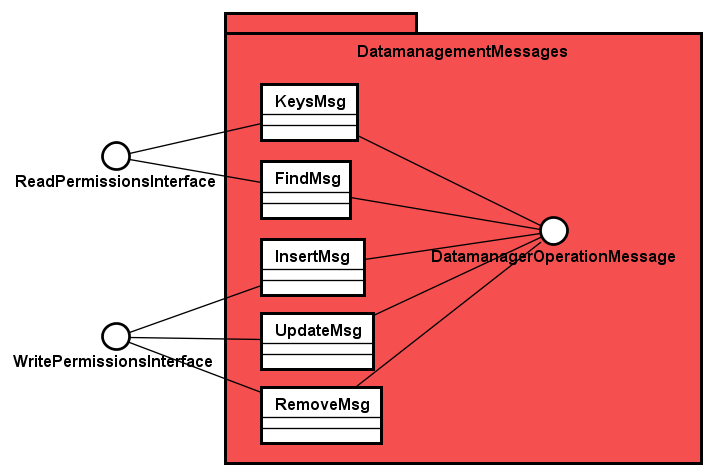
\includegraphics[scale=0.50]{Server/Package/DatamanagementMessagesLevel.png}
			\caption{Componente Actorbase.Server.Core.Messages.DatamanagementOperationMessages}
			\end{figure}
			\subsubsection{Descrizione}
				All'interno di questo package sono definite le classi e le interfacce che rappresentano messaggi relativi ad operazioni sui dati.
			\subsubsection{Classi}
			\begin{itemize}
				\item Actorbase.Server.Core.Messages.DatamanagementOperationMessages.KeysMsg
				\item Actorbase.Server.Core.Messages.DatamanagementOperationMessages.FindMsg
				\item Actorbase.Server.Core.Messages.DatamanagementOperationMessages.InsertMsg
				\item Actorbase.Server.Core.Messages.DatamanagementOperationMessages.UpdateMsg
				\item Actorbase.Server.Core.Messages.DatamanagementOperationMessages.RemoveMsg
			\end{itemize}
			\subsubsection{Interfacce}
			\begin{itemize}
				\item Actorbase.Server.Core.Messages.DatamanagementOperationMessages.DatamanagementMessage
			\end{itemize}

			\subsection{Actorbase.Server.Core.Messages.DatamanagementOperationMessages.KeysMsg}
			\subsubsection{Descrizione}
				Classe che definisce un messaggio KeysMsg.
			\subsubsection{Utilizzo}
				Un messaggio KeysMsg richiede la lista di chiavi della mappa selezionata.
			\subsubsection{Relazioni con altre classi}
			\begin{itemize}
				\item \textbf{Actorbase.Server.Core.Actors.Storefinder.MessagesBuilder:} relazione entrante, creazione
			\end{itemize}
			\subsubsection{Interfacce estese}
			\begin{itemize}
				\item Actorbase.Server.Core.Messages.DatamanagementOperationMessages.DatamanagementMessage
				\item Actorbase.Server.Core.Messages.PermissionMessages.ReadPermissionInterface
			\end{itemize}

			\subsection{Actorbase.Server.Core.Messages.DatamanagementOperationMessages.FindMsg}
			\subsubsection{Descrizione}
				Classe che definisce un messaggio FindMsg.
			\subsubsection{Utilizzo}
				Un messaggio FindMsg richiede il valore dell'item con la chiave contenuta nel messaggio.
			\subsubsection{Relazioni con altre classi}
			\begin{itemize}
				\item \textbf{Actorbase.Server.Core.Actors.Storefinder.MessagesBuilder:} relazione entrante, creazione
			\end{itemize}
			\subsubsection{Interfacce estese}
			\begin{itemize}
				\item Actorbase.Server.Core.Messages.DatamanagementOperationMessages.DatamanagementMessage
				\item Actorbase.Server.Core.Messages.PermissionMessages.ReadPermissionInterface
			\end{itemize}

			\subsection{Actorbase.Server.Core.Messages.DatamanagementOperationMessages.InsertMsg}
			\subsubsection{Descrizione}
				Classe che definisce un messaggio InsertMsg.
			\subsubsection{Utilizzo}
				Un messaggio InsertMsg richiede l'inserimento di un item con chiave e valore contenuti nel messaggio.
			\subsubsection{Relazioni con altre classi}
			\begin{itemize}
				\item \textbf{Actorbase.Server.Core.Actors.Storefinder.MessagesBuilder:} relazione entrante, creazione
			\end{itemize}
			\subsubsection{Interfacce estese}
			\begin{itemize}
				\item Actorbase.Server.Core.Messages.DatamanagementOperationMessages.DatamanagementMessage
				\item Actorbase.Server.Core.Messages.PermissionMessages.WritePermissionInterface
			\end{itemize}

			\subsection{Actorbase.Server.Core.Messages.DatamanagementOperationMessages.UpdateMsg}
			\subsubsection{Descrizione}
				Classe che definisce un messaggio UpdateMsg.
			\subsubsection{Utilizzo}
				Un messaggio UpdateMsg richiede l'aggiornamento di un item con chiave e valore contenuti nel messaggio.
			\subsubsection{Relazioni con altre classi}
			\begin{itemize}
				\item \textbf{Actorbase.Server.Core.Actors.Storefinder.MessagesBuilder:} relazione entrante, creazione
			\end{itemize}
			\subsubsection{Interfacce estese}
			\begin{itemize}
				\item Actorbase.Server.Core.Messages.DatamanagementOperationMessages.DatamanagementMessage
				\item Actorbase.Server.Core.Messages.PermissionMessages.WritePermissionInterface
			\end{itemize}

			\subsection{Actorbase.Server.Core.Messages.DatamanagementOperationMessages.DeleteMsg}
			\subsubsection{Descrizione}
				Classe che definisce un messaggio DeleteMsg.
			\subsubsection{Utilizzo}
				Un messaggio DeleteMsg richiede l'eliminazione dell'item con chiave contenuta nel messaggio.
			\subsubsection{Relazioni con altre classi}
			\begin{itemize}
				\item \textbf{Actorbase.Server.Core.Actors.Storefinder.MessagesBuilder:} relazione entrante, creazione
			\end{itemize}
			\subsubsection{Interfacce estese}
			\begin{itemize}
				\item Actorbase.Server.Core.Messages.DatamanagementOperationMessages.DatamanagementMessage
				\item Actorbase.Server.Core.Messages.PermissionMessages.WritePermissionInterface
			\end{itemize}
			
			\subsection{Actorbase.Server.Core.Messages.ChangeInterfaceMessages}
			\begin{figure} [H]
			\centering
			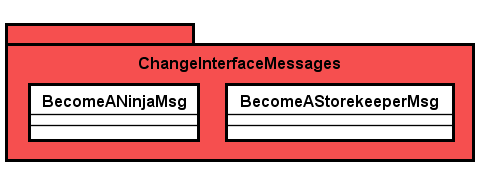
\includegraphics[scale=0.65]{Server/Package/ChangeInterfaceMessagesLevel.png}
			\caption{Componente Actorbase.Server.Core.Messages.ChangeInterfaceMessages}
			\end{figure}
			\subsubsection{Descrizione}
				All'interno di questo package sono definite le classi e le interfacce che rappresentano i messaggi inviabili per effettuare operazioni di cambio interfaccia per gli attori che supportano tale funzionalità.
			\subsubsection{Classi}
			\begin{itemize}
				\item Actorbase.Server.Core.Messages.ChangeInterfaceMessages.BecomeANinjaMsg
				\item Actorbase.Server.Core.Messages.ChangeInterfaceMessages.BecomeAStoreKeeperMsg
			\end{itemize}

			\subsection{Actorbase.Server.Core.Messages.ChangeInterfaceMessages.BecomeANinjaMsg}
			\subsubsection{Descrizione}
				Classe che definisce un messaggio BecomeANinjaMsg.
			\subsubsection{Utilizzo}
				Un messaggio BecomeANinjaMsg richiede ad un actor Datamanager di cambiare il suo comportamento in Ninja.
			\subsubsection{Relazioni con altre classi}
			\begin{itemize}
				\item \textbf{Actorbase.Server.Core.Actors.Storefinder.MessagesBuilder:} relazione entrante, creazione
			\end{itemize}

			\subsection{Actorbase.Server.Core.Messages.ChangeInterfaceMessages.\\ BecomeAStorekeeperMsg}
			\subsubsection{Descrizione}
				Classe che definisce un messaggio BecomeAStorekeeperMsg.
			\subsubsection{Utilizzo}
				Un messaggio BecomeAStorekeeperMsg richiede ad un actor Datamanager di cambiare il suo comportamento in Storekeeper.
			\subsubsection{Relazioni con altre classi}
			\begin{itemize}
				\item \textbf{Actorbase.Server.Core.Actors.Storefinder.MessagesBuilder:} relazione entrante, creazione
			\end{itemize}
			
			
					\subsection{Actorbase.Driver}
		\begin{figure} [H]
			\centering
			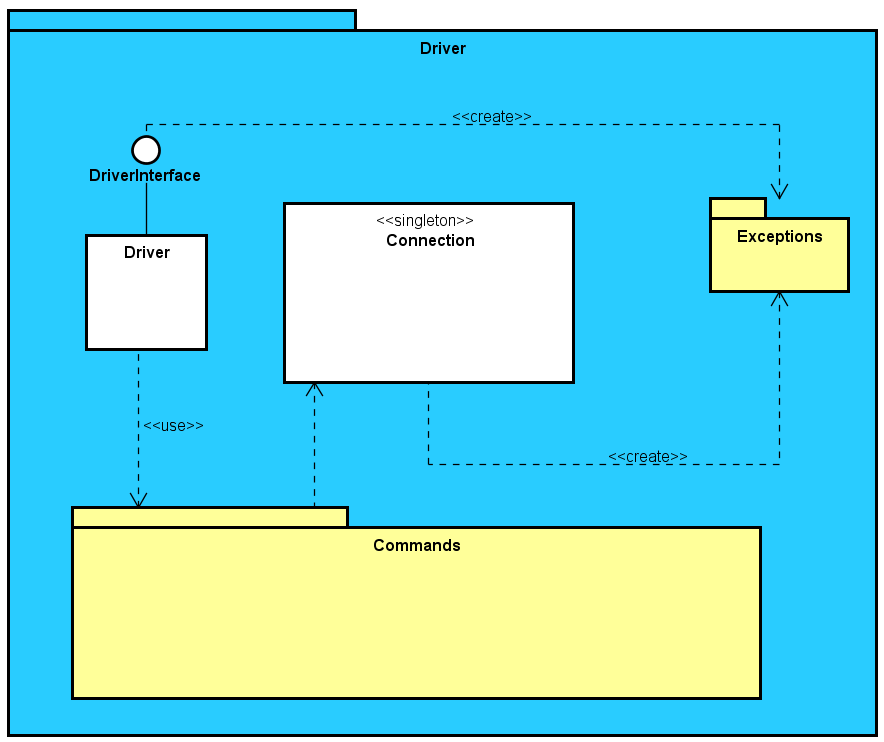
\includegraphics[scale=0.5]{ST/Client/DriverSemplificato.png}
        	\caption{Componente Actorbase.Driver}
		\end{figure}
		
		\subsubsection{Descrizione}
			Package per la componente Driver del sistema. Per la gestione dei comandi implementa il Design Pattern Command.
			
		\subsubsection{Package Figli}
			\begin{itemize}
				\item Actorbase.Driver.Components
				\item Actorbase.Driver.Exceptions
			\end{itemize}
			
		\subsubsection{Classi}
			\begin{itemize}
				\item Actorbase.Driver.Driver
				\item Actorbase.Driver.Connection
			\end{itemize}
			
		\subsubsection{Interfacce}
			\begin{itemize}
				\item Actorbase.Driver.DriverInterface
			\end{itemize}
		
		\subsection{Actorbase.Driver.Connection}
		
		\subsubsection{Descrizione}
			Classe \emph{singleton} che gestisce la comunicazione del Driver con il Server. Svolge il ruolo di \emph{Receiver}.
		\subsubsection{Utilizzo}
			Viene usata per aprire e chiudere la connessione con il Server, inviare i messaggi e per generare la prima parte del comando per le API.
		\subsubsection{Relazione con altre classi}
			\begin{itemize}
				\item \textbf{Actorbase.Driver.Commands.ServerCommand:} Relazione entrante, invio comando al Server.
				\item \textbf{Actorbase.Driver.Exception:} Relazione uscente, creazione di eccezioni.
			\end{itemize}
		
		\subsection{Actorbase.Driver.Driver}
		
		\subsubsection{Descrizione}
			Classe che gestisce la comunicazione mediante API. Svolge il ruolo di \emph{Invoker}.
		\subsubsection{Utilizzo}
			Espone i metodi per codifica e decodifica dei comandi delle API. Inoltre mantiene le informazioni relative ad eventuali Database o Mappe selezionate.
		\subsubsection{Interfacce Estese}
			Actorbase.Driver.DriverInterface
		\subsubsection{Relazioni con altre classi}
		\begin{itemize}
			\item \textbf{Actorbase.Driver.Commands:} Relazione uscente, utilizzo del metodo Execute.
			\item \textbf{Actorbase.Driver.Exceptions:} Relazione uscente, creazione di eccezioni.
		\end{itemize}
		
		
	\subsection{Actorbase.Driver.Commands}
		\begin{figure} [H]
			\centering
			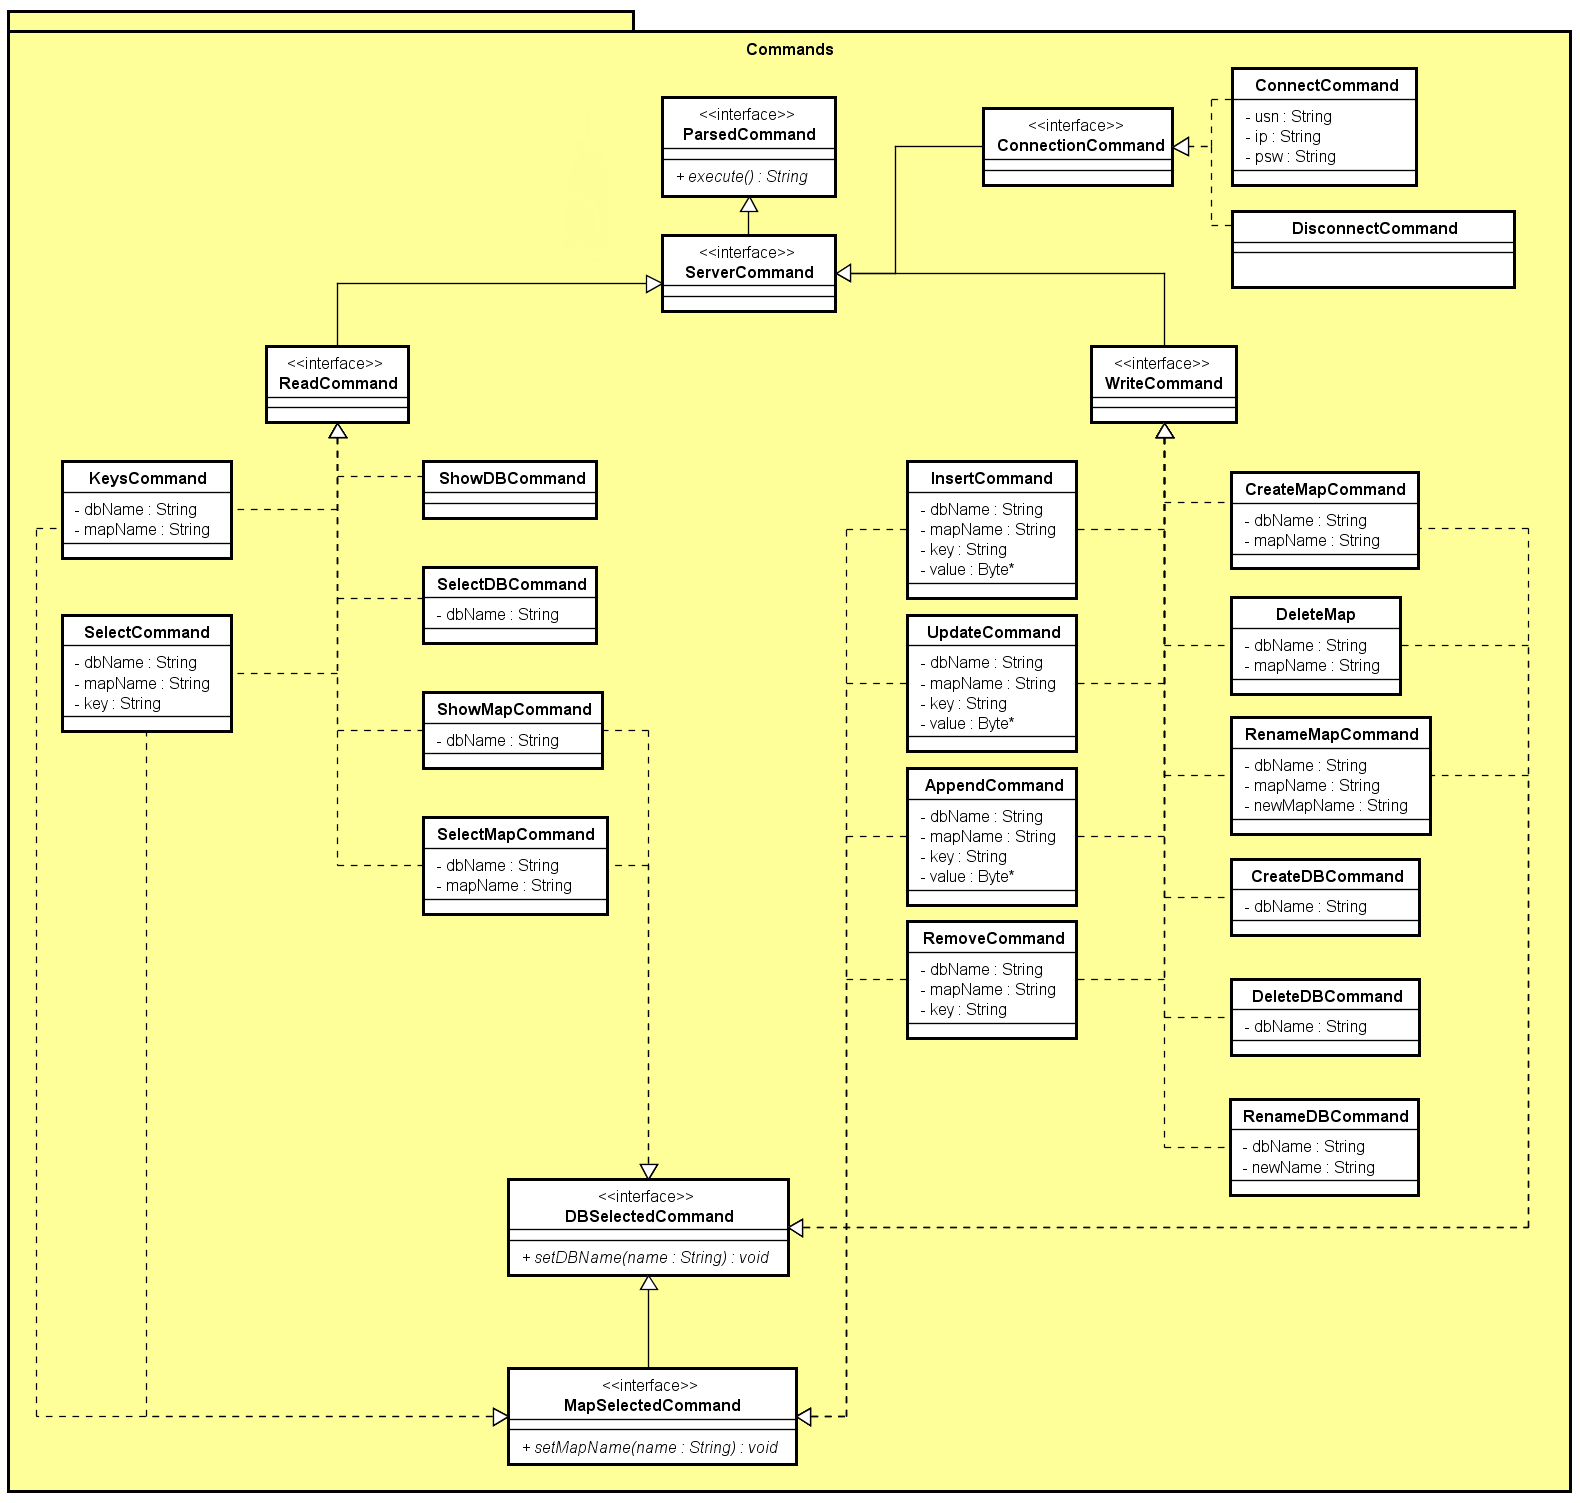
\includegraphics[scale=0.40]{ST/Client/CommandsClasses.png}
			\caption{Package Actorbase.Driver.Commands}
		\end{figure}
		\subsubsection{Descrizione}
			Package che contiene la gerarchia di comandi dell'interfaccia \emph{Command}. Ognuno di essi rappresenta astrattamente una operazione che deve essere svolta a livello del Server. Sono presenti due gerarchie di interfacce, una per la tipologia di comandi (lato client, lato server, lettura, scrittura) e l'altra per la tipologia di "pre-selezioni" necessarie per eseguire il comando (Database selezionato, Mappa selezionata).
		
		\subsubsection{Interfacce}
			\begin{itemize}
				\item Actorbase.Driver.Commands.ServerCommand
				\item Actorbase.Driver.Commands.ReadCommand
				\item Actorbase.Driver.Commands.WriteCommand
				\item Actorbase.Driver.Commands.ConnectionCommand
				\item Actorbase.Driver.Commands.DBSelectedCommand
				\item Actorbase.Driver.Commands.MapSelectedCommand
			\end{itemize}

		\subsubsection{Classi}
			\begin{itemize}
				\item Actorbase.Driver.Commands.KeysCommand
				\item Actorbase.Driver.Commands.SelectCommand
				\item Actorbase.Driver.Commands.ShowDBCommand
				\item Actorbase.Driver.Commands.SelectDBCommand
				\item Actorbase.Driver.Commands.ShowMapCommand
				\item Actorbase.Driver.Commands.SelectMapCommand
				\item Actorbase.Driver.Commands.InsertCommand
				\item Actorbase.Driver.Commands.UpdateCommand
				\item Actorbase.Driver.Commands.AppendCommand
				\item Actorbase.Driver.Commands.RemoveCommand
				\item Actorbase.Driver.Commands.CreateMapCommand
				\item Actorbase.Driver.Commands.DeleteMapCommand
				\item Actorbase.Driver.Commands.RenameMapCommand
				\item Actorbase.Driver.Commands.CreateDBCommand
				\item Actorbase.Driver.Commands.DeleteDBCommand
				\item Actorbase.Driver.Commands.RenameDBCommand
				\item Actorbase.Driver.Commands.ConnectCommand
				\item Actorbase.Driver.Commands.DisconnectCommand
			\end{itemize}
		
		\subsubsection{Relazioni con altre componenti}
			\begin{itemize}
				\item \textbf{Actorbase.Client.Model:} Relazione entrante, inclusione.
				\item \textbf{Actorbase.Client.Controller:}	Relazione entrante, inclusione.
			\end{itemize}

		

		\subsection{Actorbase.Driver.Commands.ParsedCommand}
			\subsubsection{Descrizione} Interfaccia base che rappresenta un generico comando che il Driver sa trattare.
			\subsubsection{Interfacce Figle} Actorbase.Driver.Commands.ServerCommand

		
		\subsection{Actorbase.Driver.Commands.ServerCommand}
			\subsubsection{Descrizione} Interfaccia base che rappresenta un comando lato Server.
			\subsubsection{Interfacce Estese} Actorbase.Driver.Commands.ParsedCommand
			\subsubsection{Interfacce Figlie}
				\begin{itemize}
					\item Actorbase.Driver.Commands.ReadCommand
					\item Actorbase.Driver.Commands.WriteCommand
					\item Actorbase.Driver.Commands.ConnectionCommand
				\end{itemize}
		
		\subsection{Actorbase.Driver.Commands.ReadCommand}
				\subsubsection{Descrizione} Interfaccia base che rappresenta un comando per cui sono necessari i permessi di lettura sulla tabella selezionata
				\subsubsection{Interfacce Estese} Actorbase.Driver.Commands.ServerCommand
				\subsubsection{Classi Figlie}
					\begin{itemize}
						\item \textbf{Actorbase.Driver.Commands.KeysCommand:}
							Classe concreta che rappresenta il comando per mostrare la lista delle chiavi nella mappa selezionata.
						\item \textbf{Actorbase.Driver.Commands.SelectCommand:}
							Classe concreta che rappresenta il comando per selezionare il valore di una chiave nella mappa selezionata.
						\item \textbf{Actorbase.Driver.Commands.ShowBDCommand:}
							Classe concreta che rappresenta il comando per mostrare l'elenco dei Database di cui si hanno permessi di lettura.
						\item \textbf{Actorbase.Driver.Commands.SelectDBCommand:}
							Classe concreta che rappresenta il comando per selezionare un determinato Database.
						\item \textbf{Actorbase.Driver.Commands.ShowMapCommand:}
							Classe concreta che rappresenta il comando per mostrare la lista delle mappe nel Database selezionato.
						\item \textbf{Actorbase.Driver.Commands.SelectMapCommand:}
							Classe concreta che rappresenta il comando per selezionare una determinata mappa.
					\end{itemize}


		\subsection{Actorbase.Driver.Commands.WriteCommand}
			\subsubsection{Descrizione} Interfaccia base che rappresenta un comando per cui sono necessari i permessi di scrittura sulla tabella selezionata
			\subsubsection{Interfacce Estese} Actorbase.Driver.Commands.ServerCommand
			\subsubsection{Classi Figlie}
				\begin{itemize}
					\item \textbf{Actorbase.Driver.Commands.InsertCommand:}
						Classe concreta che rappresenta il comando per inserire una coppia chiave-valore nella mappa selezionata.
					\item \textbf{Actorbase.Driver.Commands.UpdateCommand:}
						Classe concreta che rappresenta il comando per aggiornare il valore di una chiave nella mappa selezionata.
					\item \textbf{Actorbase.Driver.Commands.AppendCommand:}
						Classe concreta che rappresenta il comando per appendere in coda al valore di una chiave nella mappa selezionata.
					\item \textbf{Actorbase.Driver.Commands.RemoveCommand:}
						Classe concreta che rappresenta il comando per rimuovere una coppia chiave-valore dalla mappa selezionata.
					\item \textbf{Actorbase.Driver.Commands.CreateMapCommand:}
						Classe concreta che rappresenta il comando per creare una nuova mappa nel Database selezionato.
					\item \textbf{Actorbase.Driver.Commands.DeleteMapCommand:}
						Classe concreta che rappresenta il comando per eliminare una mappa nel Database selezionato.
					\item \textbf{Actorbase.Driver.Commands.RenameMapCommand:}
						Classe concreta che rappresenta il comando per rinominare una mappa nel Database selezionato.
					\item \textbf{Actorbase.Driver.Commands.CreateDBCommand:}
						Classe concreta che rappresenta il comando per creare un nuovo Database.
					\item \textbf{Actorbase.Driver.Commands.DeleteDBCommand:}
						Classe concreta che rappresenta il comando per rimuovere un Database.
					\item \textbf{Actorbase.Driver.Commands.RenameDBCommand:}
						Classe concreta che rappresenta il comando per rinominare un Database.
				\end{itemize}

		
		\subsection{Actorbase.Driver.Commands.ConnectionCommand}
			\subsubsection{Descrizione} Interfaccia base che rappresenta un comando di connessione o disconnessione dal Server.
			\subsubsection{Interfacce Estese} Actorbase.Driver.Commands.ServerCommand
			\subsubsection{Classi Figlie}
				\begin{itemize}
					\item \textbf{Actorbase.Driver.Commands.ConnectCommand:}
						Classe concreta che rappresenta il comando per la connessione al server.
					\item \textbf{Actorbase.Driver.Commands.DisconnectCommand:}
						Classe concreta che rappresenta il comando per la disconnessione dal server.
				\end{itemize}
		
		\subsection{Actorbase.Driver.Commands.DBSelectedCommand}
				\subsubsection{Descrizione} Interfaccia base che rappresenta un generico comando per il quale è necessario avere un Database selezionato.
				\subsubsection{Classi Figlie}
					\begin{itemize}
						\item Actorbase.Driver.Commands.ShowMapCommand
						\item Actorbase.Driver.Commands.SelectMapCommand
						\item Actorbase.Driver.Commands.CreateCommand
						\item Actorbase.Driver.Commands.DeleteCommand
						\item Actorbase.Driver.Commands.RenameCommand
					\end{itemize}


		\subsection{Actorbase.Driver.Commands.MapSelectedCommand}
				\subsubsection{Descrizione} Interfaccia base che rappresenta un generico comando per il quale è necessario avere una mappa selezionata.
				\subsubsection{Interfacce Estese} Actorbase.Driver.Commands.DBSelectedCommand
				\subsubsection{Classi Figlie}
					\begin{itemize}
						\item Actorbase.Driver.Commands.KeysCommand
						\item Actorbase.Driver.Commands.SelectCommand
						\item Actorbase.Driver.Commands.InsertCommand
						\item Actorbase.Driver.Commands.UpdateCommand
						\item Actorbase.Driver.Commands.AppendCommand
						\item Actorbase.Driver.Commands.RemoveCommand
					\end{itemize}

	
	\subsection{Actorbase.Client}
		\begin{figure} [H]
			\centering
			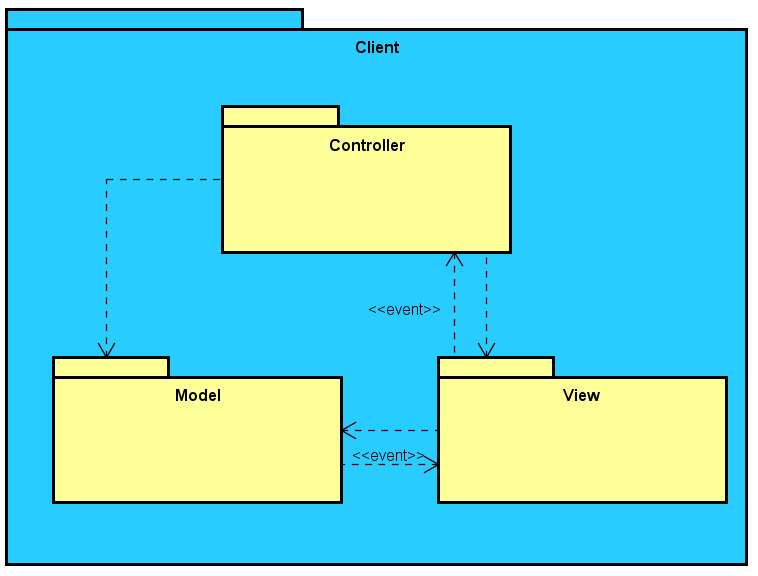
\includegraphics[scale=0.5]{ST/Client/ClientPackage.png}
        	\caption{Package Actorbase.Client}
		\end{figure}
		\subsubsection{Descrizione}
			Package per la componente Client del sistema. Implementa il Design Pattern Model View Controller.
		\subsubsection{Package Figli}
			\begin{itemize}
				\item Actorbase.Client.Model
				\item Actorbase.Client.View
				\item Actorbase.Client.Controller
			\end{itemize}
			
	\subsection{Actorbase.Client.Model}
		\begin{figure} [H]
			\centering
			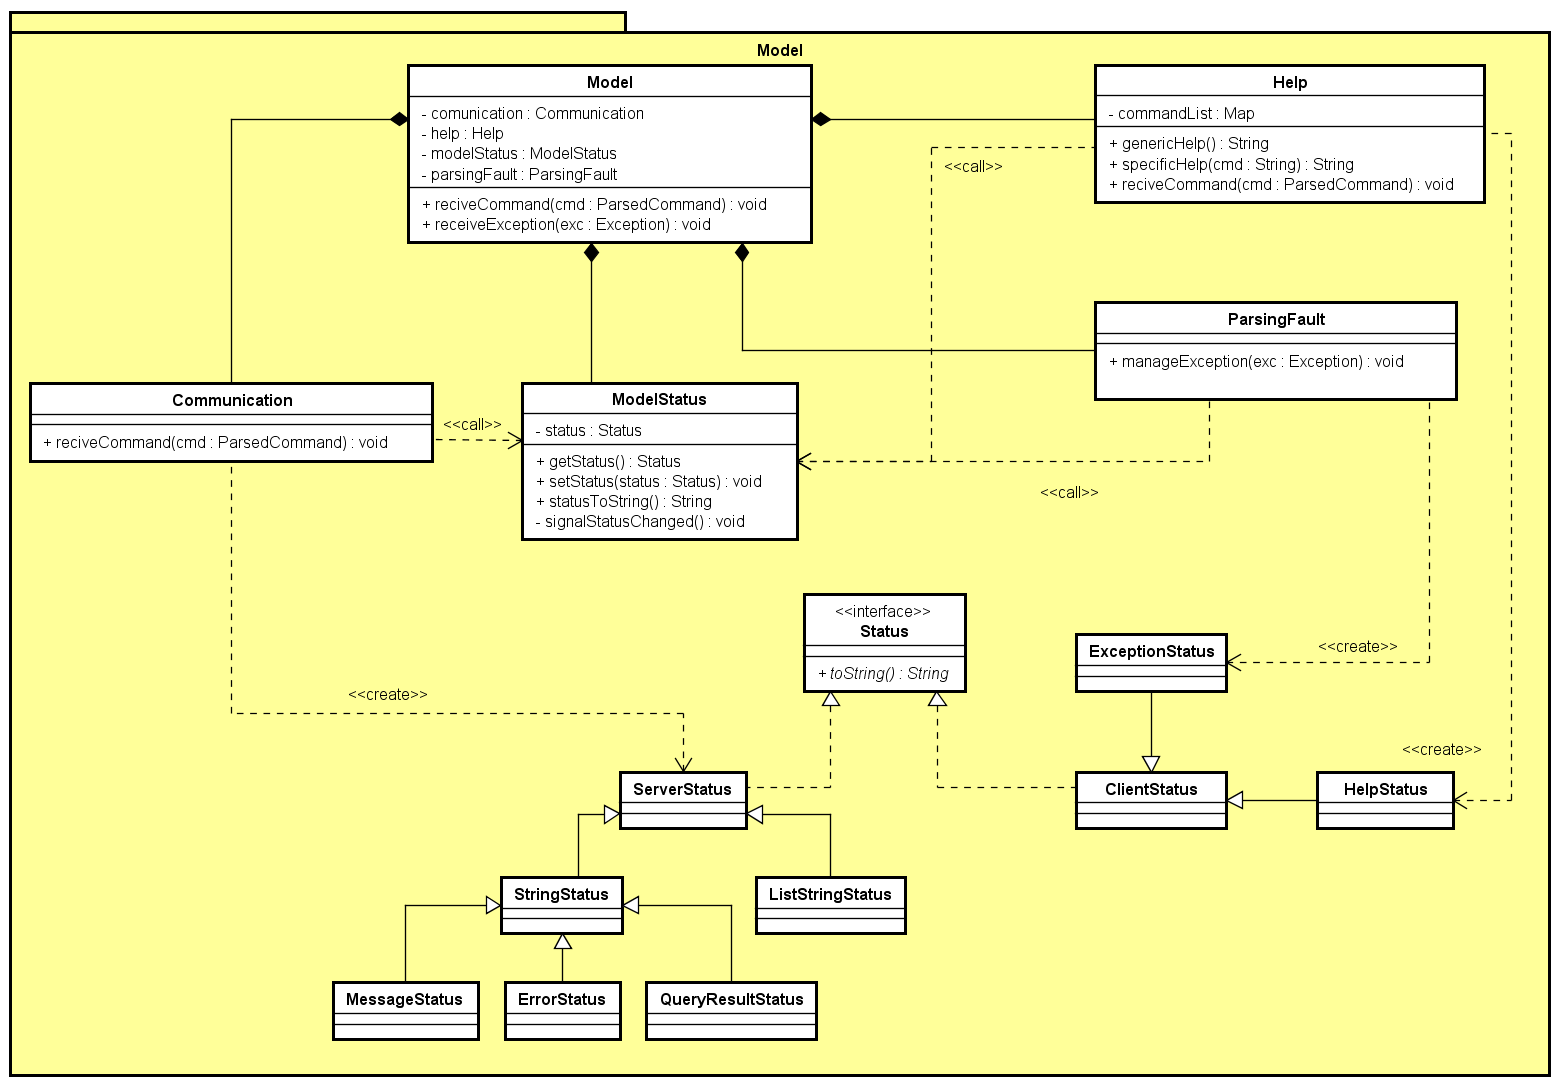
\includegraphics[scale=0.42]{ST/Client/ModelClasses.png}
        	\caption{Package Actorbase.Client.Model}
		\end{figure}
		\subsubsection{Descrizione}
			Package per la componente Model del pattern MVC della componente Client.
		\subsubsection{Interfacce}
			\begin{itemize}
				\item Actorbase.Client.Model.Status
			\end{itemize}
		\subsubsection{Classi}
			\begin{itemize}
				\item Actorbase.Client.Model.Model
				\item Actorbase.Client.Model.Help
				\item Actorbase.Client.Model.ParsingFault
				\item Actorbase.Client.Model.Comunication
				\item Actorbase.Client.Model.ModelStatus
				\item Actorbase.Client.Model.ServerStatus
				\item Actorbase.Client.Model.StringStatus
				\item Actorbase.Client.Model.ListStringStatus
				\item Actorbase.Client.Model.MessageErrorStatus
				\item Actorbase.Client.Model.QueryResultStatus
				\item Actorbase.Client.Model.ExceptionStatus
				\item Actorbase.Client.Model.HelpStatus
			\end{itemize}
		\subsubsection{Relazioni con altre componenti}
				\begin{itemize}
					\item \textbf{Actorbase.Driver.Commands:} Relazione uscente, inclusione.
				\end{itemize}	
		
		\subsection{Actorbase.Client.Model.Status}
			\subsubsection{Descrizione}
				Interfaccia base della gerarchia degli stati del Model.
			\subsubsection{Utilizzo}
				Rappresenta un generico stato che il Model può assumere, è la rappresentazione astratta della frazione di stato dell'intero sistema Actorbase che è richiesta dall'utente. Le sue classi figlie espongono tutte un metodo per poter restituire in forma di stringa le informazioni alla View.
			\subsubsection{Classi Figlie}
				\begin{itemize}
					\item Actorbase.Client.Model.ServerStatus
					\item Actorbase.Client.Model.ClientStatus		
				\end{itemize}
			
		\subsection{Actorbase.Client.Model.ServerStatus}
			\subsubsection{Descrizione}
				Classe base per un generico stato restituito dal Server.
			\subsubsection{Utilizzo}
				Rappresenta un generico stato del Server che il Model può assumere.
			\subsubsection{Interfacce Estese}
				Actorbase.Client.Model.Status
			\subsubsection{Relazioni con altre classi}
				\begin{itemize}
					\item \textbf{Actorbase.Client.Model.Communication:} Relazione entrante, creazione.
				\end{itemize}
			\subsubsection{Classi Figlie}
				\begin{itemize}
					\item \textbf{Actorbase.Client.Model.ListStringStatus:}
						Stato che rappresenta un generico stato di tipo lista di stringhe.
					\item \textbf{Actorbase.Client.Model.StringStatus:}
						Stato che rappresenta un generico stato di tipo stringa.
					\begin{itemize}
						\item \textbf{Actorbase.Client.Model.MessageStatus:}
							Stato che rappresenta un messaggio del server.
						\item \textbf{Actorbase.Client.Model.ErrorStatus:}
							Stato che rappresenta un errore a livello del server.
						\item \textbf{Actorbase.Client.Model.QueryResultStatus:}
							Stato che rappresenta il risultato di una query ritornato in forma di stringa.
					\end{itemize}
				\end{itemize}
				
			
		\subsubsection{Actorbase.Client.Model.ClientStatus}
			\subsubsection{Descrizione}
				Classe base per un generico stato restituito dal Client stesso.
			\subsubsection{Utilizzo}
				Rappresenta un generico stato del Client che il Model può assumere.
			\subsubsection{Interfacce Estese}
				Actorbase.Client.Model.Status
			\subsubsection{Relazioni con altre classi}
				\begin{itemize}
					\item \textbf{Actorbase.Client.Model.Help:} Relazione entrante, creazione.
					\item \textbf{Actorbase.Client.Model.ParsingFault:} Relazione entrante, creazione.
				\end{itemize}
			\subsubsection{Classi Figlie}
				\begin{itemize}
					\item \textbf{Actorbase.Client.Model.ExceptionStatus:}
						Stato che rappresenta una eccezione.
					\item \textbf{Actorbase.Client.Model.HelpStatus:}
						Stato che rappresenta una richiesta di help da parte dell'utente.
				\end{itemize}
			
		\subsection{Actorbase.Client.Model.Model}
			\subsubsection{Descrizione}
				Classe base per la componente Model del Pattern MVC della componente Client.
			\subsubsection{Utilizzo}
				Fornisce un accesso unico al sottosistema delle classi ad esso composte.
			\subsubsection{Relazioni con altre classi}
				\begin{itemize}
					\item \textbf{Actorbase.Client.Model.Communication:} Relazione uscente, composizione.
					\item \textbf{Actorbase.Client.Model.ModelStatus:} Relazione uscente, composizione.
					\item \textbf{Actorbase.Client.Model.Help:} Relazione uscente, composizione.
					\item \textbf{Actorbase.Client.Model.ParsingFault:}	Relazione uscente, composizione.
					\item \textbf{Actorbase.Client.Controller:}	Relazione entrante, chiamata metodo per la ricezione del comando.	
				\end{itemize}
			
		\subsection{Actorbase.Client.Model.Comunication}
			\subsubsection{Descrizione}
				Classe che gestisce la comunicazione con il server tramite Driver.
			\subsubsection{Utilizzo}
				Gestisce la comunicazione con il server tramite Driver, crea gli ServerStatus e chiama il metodo per modificare l'attributo status del Model.
			\subsubsection{Relazioni con altre classi}
				\begin{itemize}
					\item \textbf{Actorbase.Client.Model.Model:} Relazione entrante, composizione.
					\item \textbf{Actorbase.Client.Model.ServerStatus:} Relazione uscente, creazione.
					\item \textbf{Actorbase.Client.Model.ModelStatus:} Relazione uscente, impostazione dello status.
					\item \textbf{Actorbase.Driver.Driver:} Relazione uscente, composizione.
				\end{itemize}
		
		\subsection{Actorbase.Client.Model.ModelStatus}
			\subsubsection{Descrizione}
				Classe che gestisce l'attributo stato di Model.
			\subsubsection{Relazioni con altre classi}
				\begin{itemize}
					\item \textbf{Actorbase.Client.Model.Model:} Relazione entrante, composizione.
					\item \textbf{Actorbase.Client.Model.Communication:} Relazione entrante, impostazione dello status.
					\item \textbf{Actorbase.Client.Model.Help:} Relazione entrante, impostazione dello status.
					\item \textbf{Actorbase.Client.Model.ParsingFault:}	Relazione entrante, impostazione dello status.
				\end{itemize}
				
		\subsection{Actorbase.Client.Model.Help}
			\subsubsection{Descrizione}
				Classe che gestisce le richieste di aiuto.
			\subsubsection{Utilizzo}
				Gestisce le richieste di aiuto, crea gli HelpStatus e chiama il metodo per modificare l'attributo status del Model.
			\subsubsection{Relazioni con altre classi}
				\begin{itemize}
					\item \textbf{Actorbase.Client.Model.Model:} Relazione entrante, composizione.
					\item \textbf{Actorbase.Client.Model.HelpStatus:} Relazione uscente, creazione.
					\item \textbf{Actorbase.Client.Model.ModelStatus:} Relazione uscente, impostazione dello status.
				\end{itemize}
				
		\subsection{Actorbase.Client.Model.ParsingFault}
			\subsubsection{Descrizione}
				Classe che gestisce le eccezioni.
			\subsubsection{Utilizzo}
				Gestisce le eccezioni, crea gli ExceptionStatus e chiama il metodo per modificare l'attributo status del Model.
			\subsubsection{Relazioni con altre classi}
				\begin{itemize}
					\item \textbf{Actorbase.Client.Model.Model:} Relazione entrante, composizione.
					\item \textbf{Actorbase.Client.Model.ExceptionStatus:} Relazione uscente, creazione.
					\item \textbf{Actorbase.Client.Model.ModelStatus:} Relazione uscente, impostazione dello status.
				\end{itemize}
		
		\subsection{Actorbase.Client.View}
			\begin{figure} [H]
				\centering
				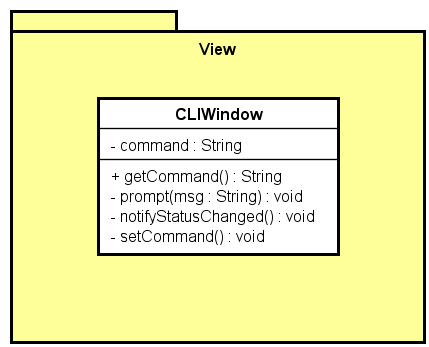
\includegraphics[scale=0.6]{ST/Client/ViewClasses.png}
   		     	\caption{Package Actorbase.Client.View}
			\end{figure}
			
			\subsubsection{Descrizione}
				Package per la componente View del pattern MVC della componente Client.
			\subsubsection{Classi}
				Actorbase.Client.View.View

		
		\subsection{Actorbase.Client.View.View}	
			\subsubsection{Descrizione}
				Classe che gestisce l'interfaccia utente.
			\subsubsection{Utilizzo}
				Gestisce l'interfaccia utente, permette di inserire comandi e stamparne l'output a video.
			\subsubsection{Relazioni con altre classi}
				\begin{itemize}
					\item \textbf{Actorbase.Client.Controller.Controller:} Relazione entrante, richiesta comando inserito.
					\item \textbf{Actorbase.Client.Controller.Controller:} Relazione uscente, segnalazione di cambio di stato.
					\item \textbf{Actorbase.Client.Model.Model:} Relazione entrante, ricezione segnale di cambio di stato.
					\item \textbf{Actorbase.Client.Model.Model:} Relazione uscente, query sullo stato del Model.
				\end{itemize}
				
				
				
		\subsection{Actorbase.Client.Controller}
			\begin{figure} [H]
				\centering
				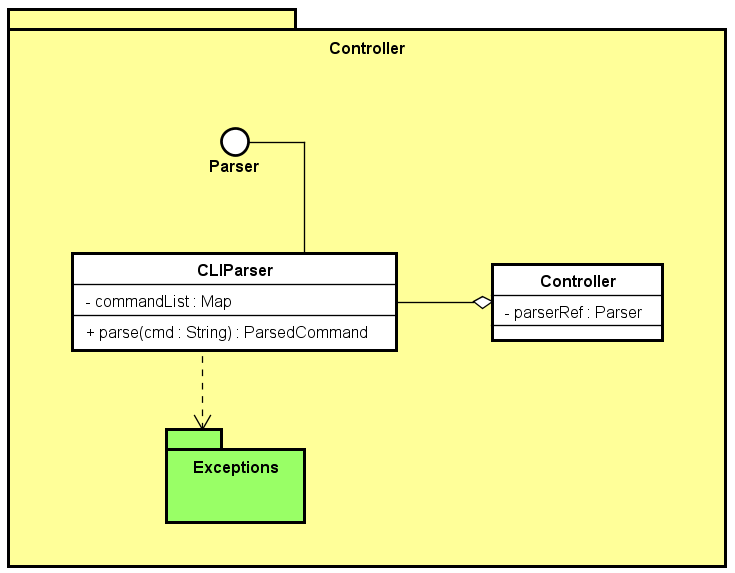
\includegraphics[scale=0.6]{ST/Client/ControllerSemplificato.png}
   		     	\caption{Package Actorbase.Client.Controller}
			\end{figure}
			
			\subsubsection{Descrizione}
				Package per la componente Controller del pattern MVC della componente Client.
			\subsubsection{Interfacce}
				Actorbase.Client.Controller.Parser
			\subsubsection{Classi}
				\begin{itemize}
					\item Actorbase.Client.Controller.CLIParser
					\item Actorbase.Client.Controller.Controller		
				\end{itemize}
			\subsubsection{Package Figli}
				Actorbase.Client.Controller.Exceptions
			\subsubsection{Relazioni con altre componenti}
				\begin{itemize}
					\item \textbf{Actorbase.Driver.Commands:} Relazione uscente, inclusione.
				\end{itemize}								
					
		\subsection{Actorbase.Client.Controller.Parser}
			\subsubsection{Descrizione}
				Interfaccia base per la gerarchia dei parser.
			\subsubsection{Utilizzo}
				Fornisce una interfaccia comune a qualsiasi parser.
			\subsubsection{Relazioni con altre classi}
				\begin{itemize}
					\item \textbf{Actorbase.Client.Controller.ClIParser:} Relazione entrante, realizzazione di interfaccia.
				\end{itemize}
		
		\subsection{Actorbase.Client.Controller.CLIParser}
			\subsubsection{Descrizione}
				Classe concreta che rappresenta un parser della DSL di Actorbase.
			\subsubsection{Utilizzo}
				Mantiene una mappa dei comandi e delle relative norme, è in grado di trasformare un comando DSL inserito dall'utente nel rispettivo comando della gerarchia Actorbase.Driver.Commands.
			\subsubsection{Relazioni con altre classi}
				\begin{itemize}
					\item \textbf{Actorbase.Client.Controller.Parser:} Relazione entrante, realizzazione di interfaccia.
					\item \textbf{Actorbase.Client.Controller.Controller:} Relazione entrante, aggregazione.
					\item \textbf{Actorbase.Client.Controller.Exception:} Relazione uscente, importazione, crea le classi presenti nel package.
				\end{itemize}
				
				
		\subsection{Actorbase.Client.Controller.Controller}
			\subsubsection{Descrizione}
				Classe base per la componente Controller del Pattern MVC della componente Client.
			\subsubsection{Utilizzo}
				Viene notificata dalla View quando il suo stato cambia, si occupa di leggere il nuovo stato della View e modificare lo status del Model.
			\subsubsection{Relazioni con altre classi}
				\begin{itemize}
					\item \textbf{Actorbase.Client.Controller.ClIParser:} Relazione uscente, aggregazione.
					\item \textbf{Actorbase.Client.View.View:} Relazione uscente, query sullo stato.
					\item \textbf{Actorbase.Client.View.View:} Relazione entrate, segnalazione di cambio stato.
					\item \textbf{Actorbase.Client.Model.Model:} Relazione uscente, cambio stato.
				\end{itemize}
				
		\subsection{Actorbase.Client.Controller.Exception}
			\begin{figure} [H]
				\centering
				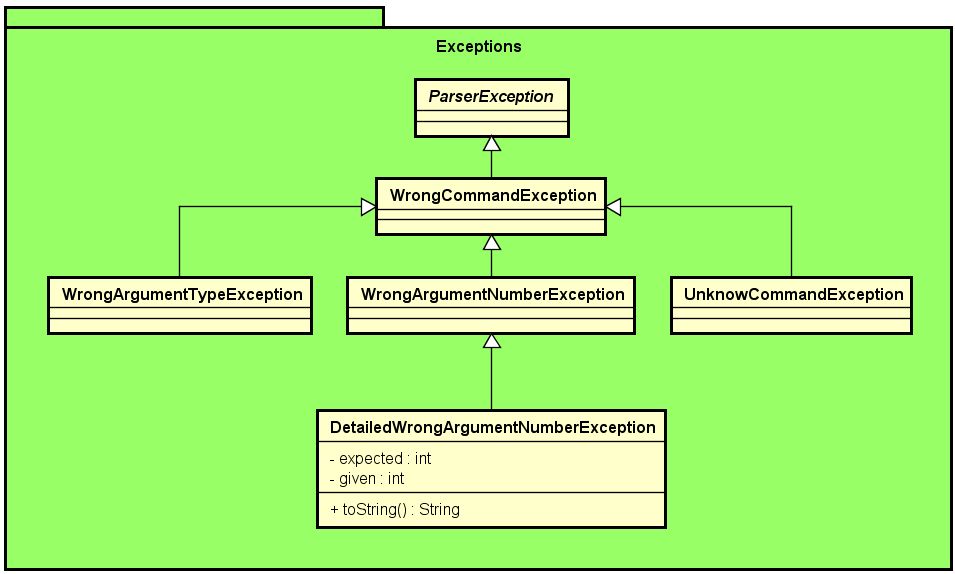
\includegraphics[scale=0.6]{ST/Client/ControllerExceptions.png}
   		     	\caption{Package Actorbase.Client.Exceptions}
			\end{figure}
			\subsubsection{Descrizione}
				Package che contiene le eccezioni che il Parser può lanciare.
			\subsubsection{Classi}
				\begin{itemize}
					\item \textbf{Actorbase.Client.Controller.Exceptions.ParserException:}
						Generica eccezione che può essere lanciata dal Parser.
					\begin{itemize}
						\item \textbf{Actorbase.Client.Controller.Exceptions.WrongCommandException:}
							Generica eccezione riguardante l'errata sintassi del comando.
						\begin{itemize}
							\item \textbf{Actorbase.Client.Controller.Exceptions.WrongArgumentTypeException:}
								Eccezione lanciata nel caso in cui il tipo dell'argomento sia errato.
							\item \textbf{Actorbase.Client.Controller.Exceptions.UnknownCommandException:}
								Eccezione lanciata nel caso in cui il comando inserito sia inesistente.
							\item \textbf{Actorbase.Client.Controller.Exceptions.WrongArgumentNumberException:}
								Eccezione lanciata nel caso in cui ci sia un numero errato di parametri per il comando inserito.
								\begin{itemize}
									\item \textbf{Actorbase.Client.Controller.Exceptions.DetailedWrongArgumentNumberException:}
										Eccezione lanciata nel caso in cui ci sia un numero errato di parametri per il comando inserito; fornisce anche il numero di parametri atteso e quello dei parametri inseriti dall'utente.
								\end{itemize}
						\end{itemize}						 
					\end{itemize}
				\end{itemize}
							 
	
	\newpage 
	\section{Diagrammi delle attività}
		Segue la descrizione dei diagrammi delle attività che mostrano le possibili interazioni dell'utente con Actorbase. Il diagramma iniziale illustrerà le attività possibili che saranno successivamente mostrate in sotto diagrammi specifici, queste attività sono segnate nel diagramma principale con un fork.
		\subsubsection{Diagramma attività principale}
		
		\begin{figure} [H]
			\centering
			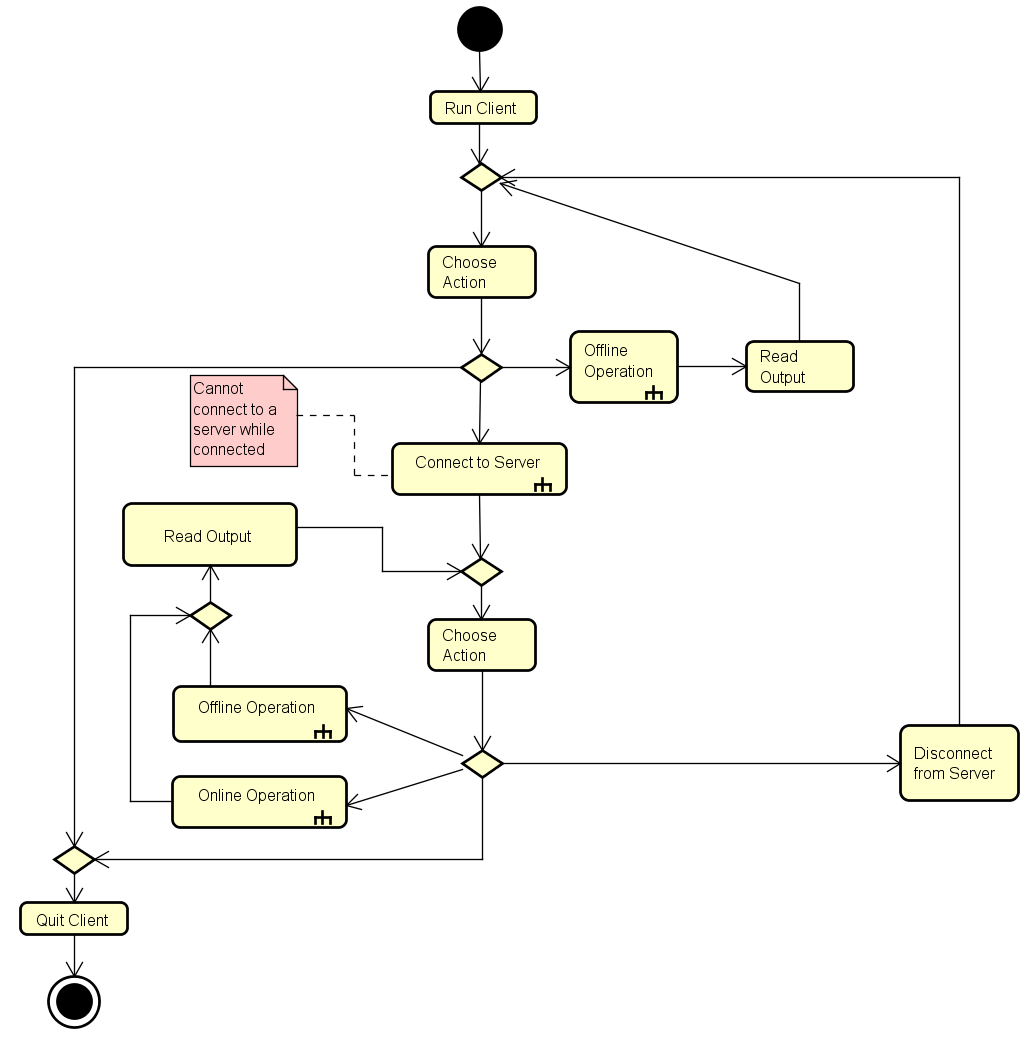
\includegraphics[scale=0.6]{ST/client/diagramma-attivita-generale.png}
			\caption{Diagramma attività principale}
		\end{figure}
			Dopo aver avviato il client l'utente può svolgere tre tipi di operazione: connettersi ad un server, chiudere l'applicativo o svolgere un'operazione offline. Se sceglie di connettersi può sempre chiudere l'applicativo e svolgere operazioni che non necessitano di essere connessi al server, può in più disconnettersi o svolgere operazioni sul server, non potrà però più connettersi ad un server finché non effettua la disconnessione dal server corrente.
			
		\subsubsection{Offline Operation}
			\begin{figure} [H]
				\centering
				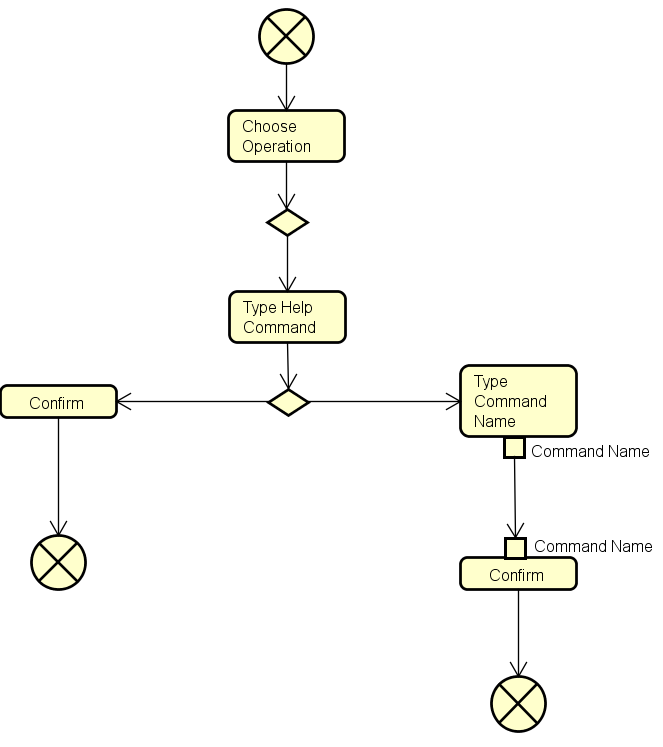
\includegraphics[scale=0.6]{ST/client/diagramma-offline-operation.png}
				\caption{Diagramma attività operazioni offline}
			\end{figure}
				L'utente sceglie se chiedere un aiuto generale, o riguardante un comando specifico, nel primo caso è sufficiente che digiti il comando di aiuto e lo confermi, altrimenti dovrà successivamente scrivere il comando del quale vuole avere chiarimenti e poi confermare.
		\subsubsection{Connect to Server}
			\begin{figure} [H]
				\centering
				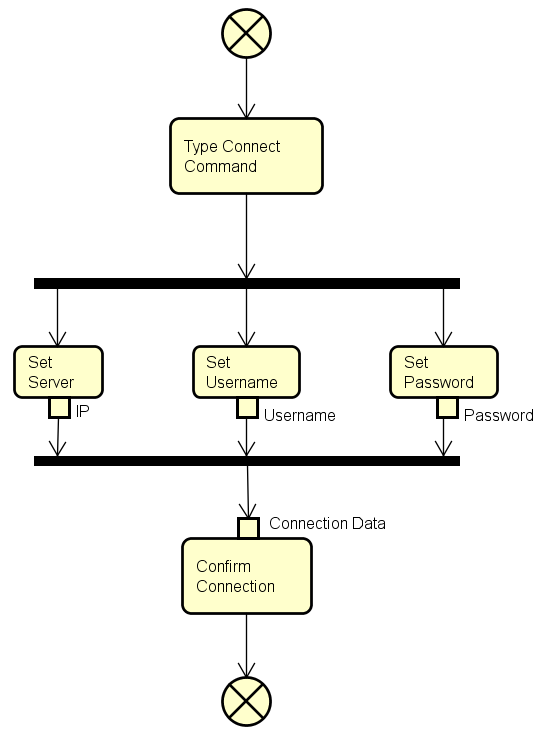
\includegraphics[scale=0.6]{ST/client/diagramma-Connect-to-Server.png}
				\caption{Diagramma attività connessione ad un server}
			\end{figure}
				Per effettuare una connessione l'utente dovrà digitare il commando di connessione e successivamente fornire i dati per la connessione, nello specifico: l'indirizzo IP al quale ci si vuole connettere, il nome utente e la password. Dopo di che è sufficiente che confermi il comando.
		\subsubsection{Online Operation}
			\begin{figure} [H]
				\centering
				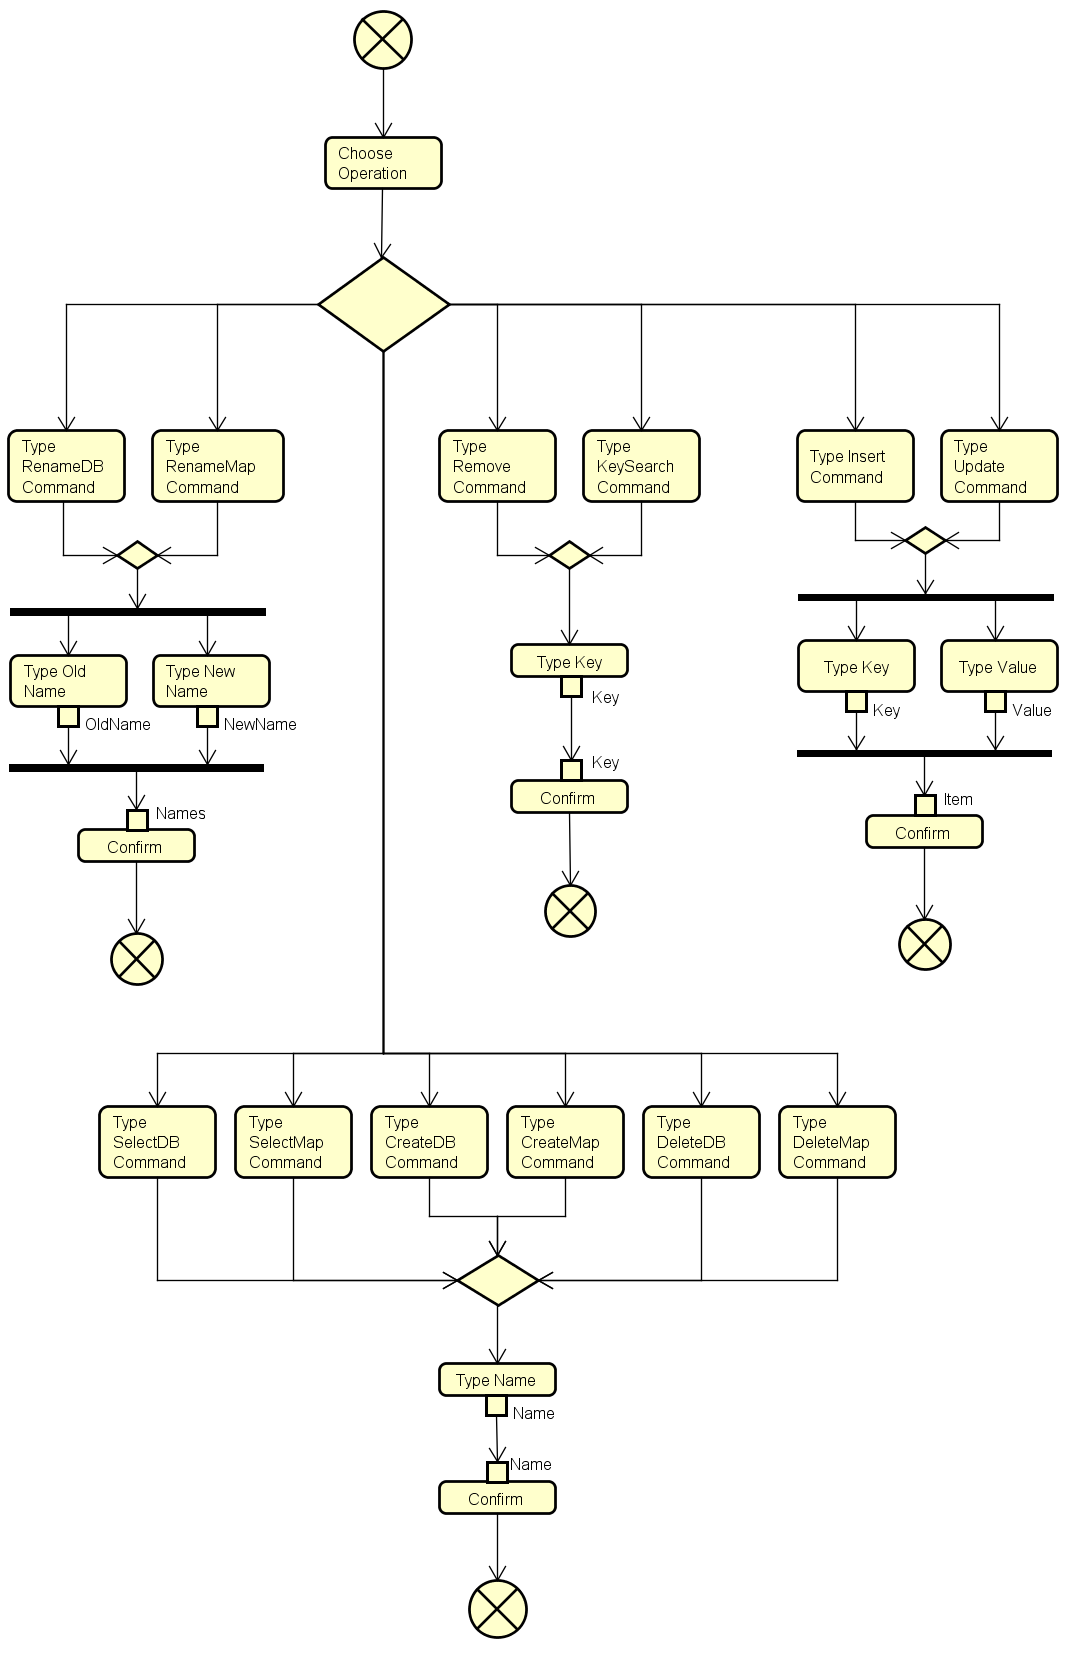
\includegraphics[scale=0.4]{ST/client/diagramma-Online-Operation.png}
				\caption{Diagramma attività operazioni online}
			\end{figure}
				L'utente sceglie che tipo di operazione vuole effettuare, se vuole effettuare un' operazione di rinomina su un Database o una mappa è sufficiente che fornisca il comando di rinomina, il vecchio e il nuovo nome e che poi confermi l'operazione; se vuole effettuare un' operazione di selezione o di creazione o di cancellazione sia di un Database che di una mappa, deve digitare il comando corretto e successivamente il nome del Database o della mappa sulla quale vuole effettuare l'operazione dopo di che è sufficiente che confermi il comando; se vuole effettuare un' operazione di rimozione o selezione di un dato è necessario che digiti il comando desiderato, digiti la chiave completa e che confermi l'operazione; se vuole effettuare un inserimento di un dato o un aggiornamento di un dato deve inserire il comando corretto, digitare la chiave completa e confermare l'operazione.
                
                
	\newpage 
	\section{Diagrammi di sequenza}
        In questa sezione verranno illustrati e descritti i principali diagrammi di sequenza realizzati. Questi ultimi illustrano ad alto livello le azioni 
        compiute dal server e dal client per gestire tutte le richieste di un utente.
        
        Per esplicitare l'invio di un messaggio tra due attori, nei diagrammi viene chiamato il metodo \textit{receive()} dell'attore che riceve il messaggio 
        da parte di chi lo invia.
        Questo è dovuto al fatto che tutte le classi ereditano dall'interfaccia \textit{Actor} messa a disposizione da \textit{Akka} senza effettuare 
        l'override del metodo per inviare i messaggi; mentre sovrascrivono il metodo di ricezione per gestire i messaggi in entrata.
        
        Trattandosi di diagrammi di sequenza non molto specifici, alcuni attori effettuano operazioni senza chiamare dei metodi specifici già 
        dichiarati. Un esempio si può vedere nel diagramma riguardante la chiusura, in esso infatti, tutti gli attori effettuano una chiamata ad un metodo 
        \textit{chiusura()}.
       
       \subsection{Avvio}
            \begin{figure} [H]
				\centering
				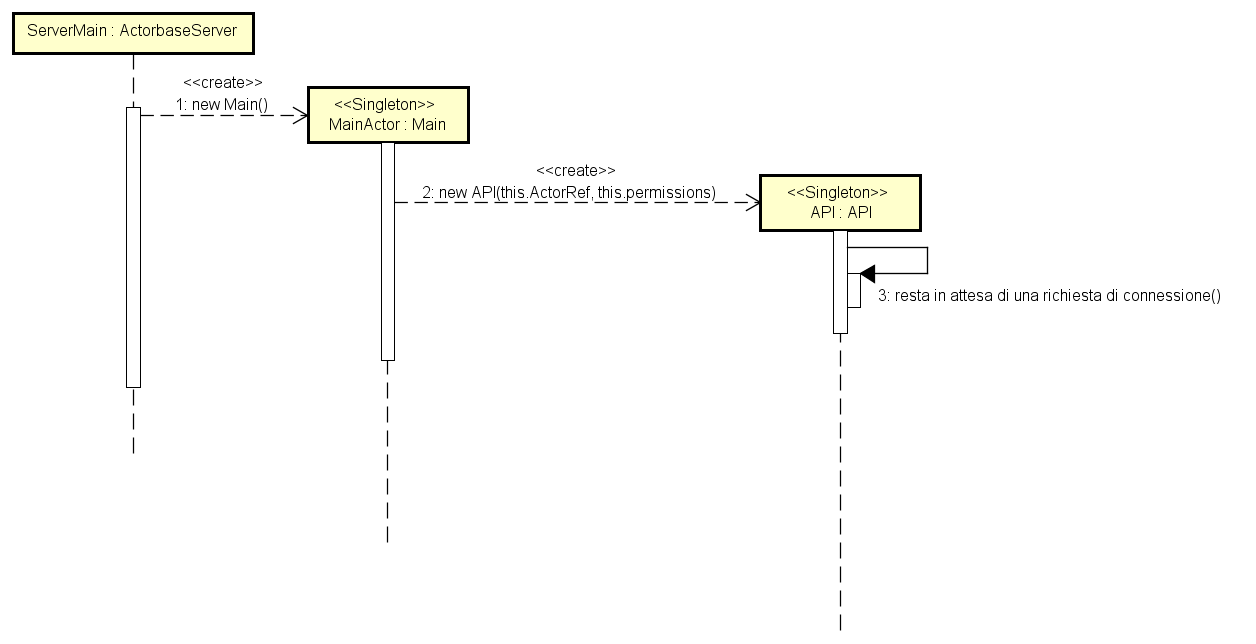
\includegraphics[width=\textwidth]{ST/seq/AvvioMain.png}
				\caption{Diagramma di sequenza - avvio del server principale.}
			\end{figure}
            Nel diagramma precedente è possibile visualizzare quali sono le operazioni che vengono eseguite per avviare il server. Esse partono dall'apertura 
            della shell, ed effettuano le prime operazioni necessarie avviando gli attori Main e API.
             
       \subsection{Chiusura}
            \begin{figure} [H]
				\centering
				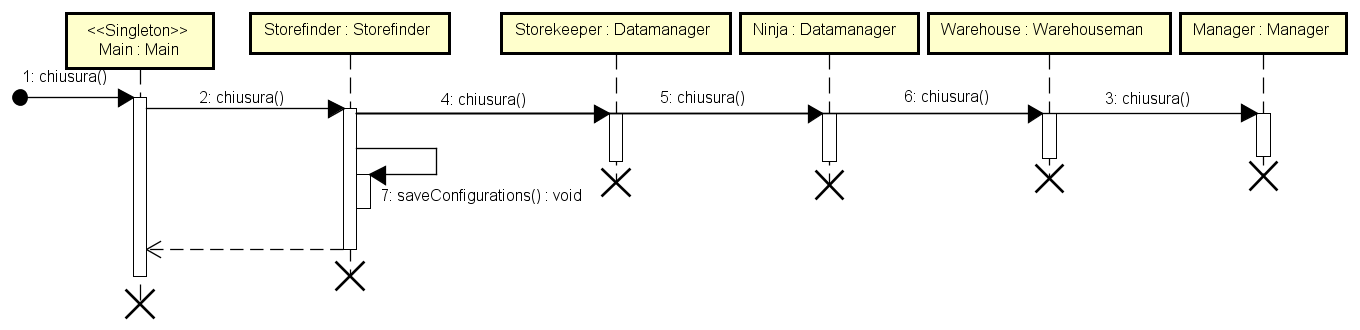
\includegraphics[width=\textwidth]{ST/seq/Chiusura.png}
				\caption{Diagramma di sequenza - chiusura del server.}
			\end{figure}
            Nel diagramma precedente è possibile visualizzare quali sono le operazioni che vengono eseguite alla chiusura del server. La classe ActorbaseServer 
            quando viene inserito il comando di chiusura del server dalla shell di comando, chiude l'attore Main, che a sua volta, chiude tutti i suoi attori 
            figli tramite il metodo di chiusura messo a disposizione dalla libreria \textit{Akka}. Una volta chiusi tutti i suoi figli (nel diagramma è espresso 
            con l'invio di una richiesta di \textit{chiusura} ai suoi figli), l'attore Main termina, effettuando i salvataggi delle configurazioni necessarie.
            
        \subsection{Richiesta esterna}
            \begin{figure} [H]
				\centering
				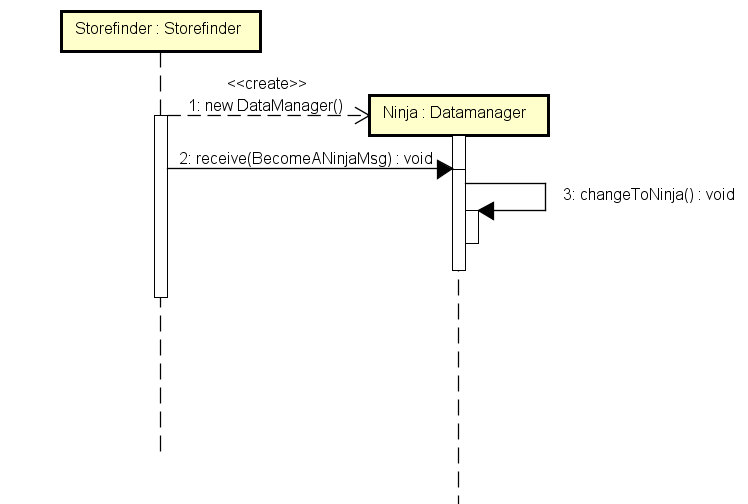
\includegraphics[width=\textwidth]{ST/seq/CreazioneNinja.png}
				\caption{Diagramma di sequenza - gestione di richiesta esterna ad alto livello.}
			\end{figure}
            Nel diagramma precedente è possibile visualizzare quali sono le operazioni che vengono eseguite da quando le API ricevono una richiesta da un client 
            esterno. Le API inviano la richiesta HTTP all'attore Main, che crea un attore MessagesBuilder che interpreta il messaggio, genera un messaggio tra quelli 
            definiti nel package \textbf{Actorbase.Server.Core.Messages} e lo restituisce tramite una future al Main. Una volta ricevuta la risposta, l'attore Main 
            gestisce il messaggio (nei diagrammi seguenti vengono specificate più nel dettaglio le operazioni effettuate in base al tipo di messaggio ricevuto). 
            Una volta terminata la gestione del messaggio, crea un HTTPBuilder a cui manda la risposta da trasformare in HTTP, una volta trasformata la rimanda 
            alle API, che la restituiscono al Client che ha effettuato la richiesta.
            
        \subsection{Richiesta di creazione DB}
            \begin{figure} [H]
				\centering
				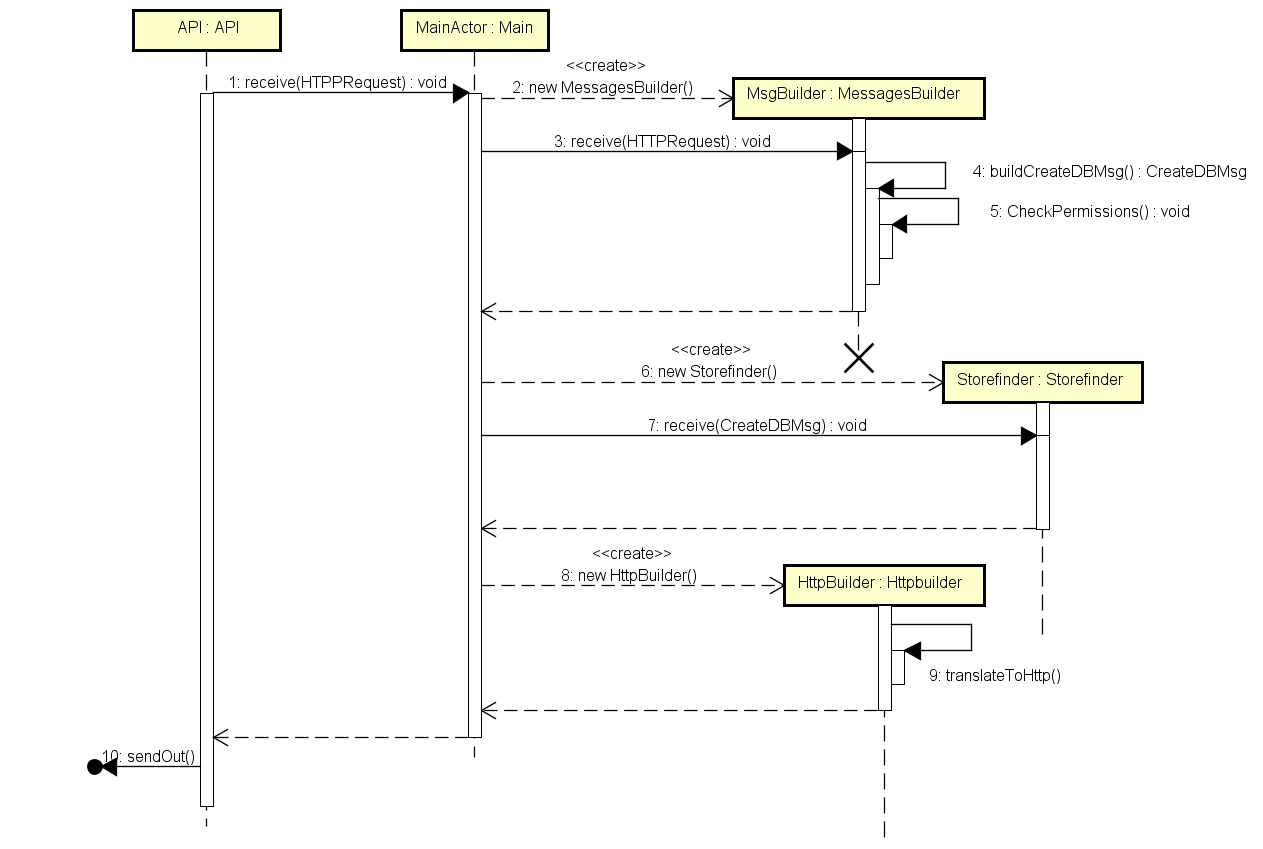
\includegraphics[width=\textwidth]{ST/seq/GestioneDB.png}
				\caption{Diagramma di sequenza - gestione di richiesta di creazione DB.}
			\end{figure}
            Nel diagramma precedente è possibile visualizzare quali sono le operazioni che vengono eseguite quando il Main riceve una richiesta di creazione di un DB.
            Come illustrato nella sezione precedente, viene trasformata la richiesta HTTP in un messaggio tramite un attore MessagesBuilder. Una volta ricevuto questo 
            messaggio, l'attore Main crea un attore Storefinder a cui assegna quel DB. Genera la risposta da restituire al Client tramite HTTPBuilder e la spedisce 
            all'esterno tramite API.
            
        \subsection{Richiesta di find}
            \begin{figure} [H]
				\centering
				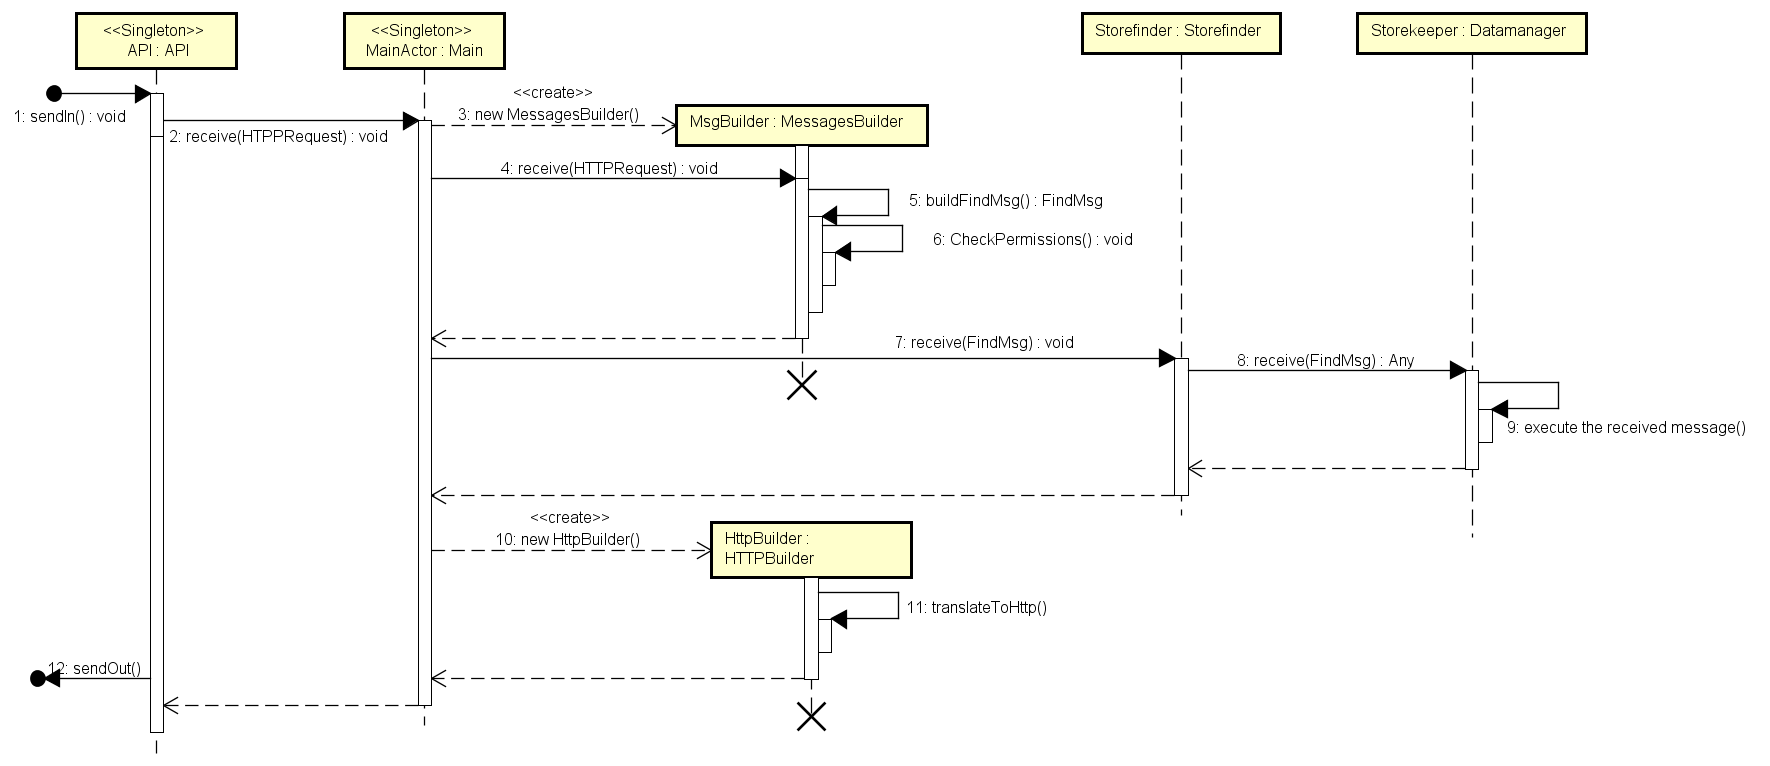
\includegraphics[width=\textwidth]{ST/seq/GestioneFind.png}
				\caption{Diagramma di sequenza - gestione di richiesta di Find.}
			\end{figure}
            Nel diagramma precedente è possibile visualizzare quali sono le operazioni che vengono eseguite per gestire una richiesta di find. L'attore Main instrada 
            il messaggio all'attore Storefinder corrispondente, il quale inoltra la richiesta all'attore Storekeeper di competenza, che interpreta la sua mappa e 
            restituisce la risposta. L'attore Main risponde alle API come specificato nei diagrammi precedenti.
            
        \subsection{Richiesta di aggiornamento item}
            \begin{figure} [H]
				\centering
				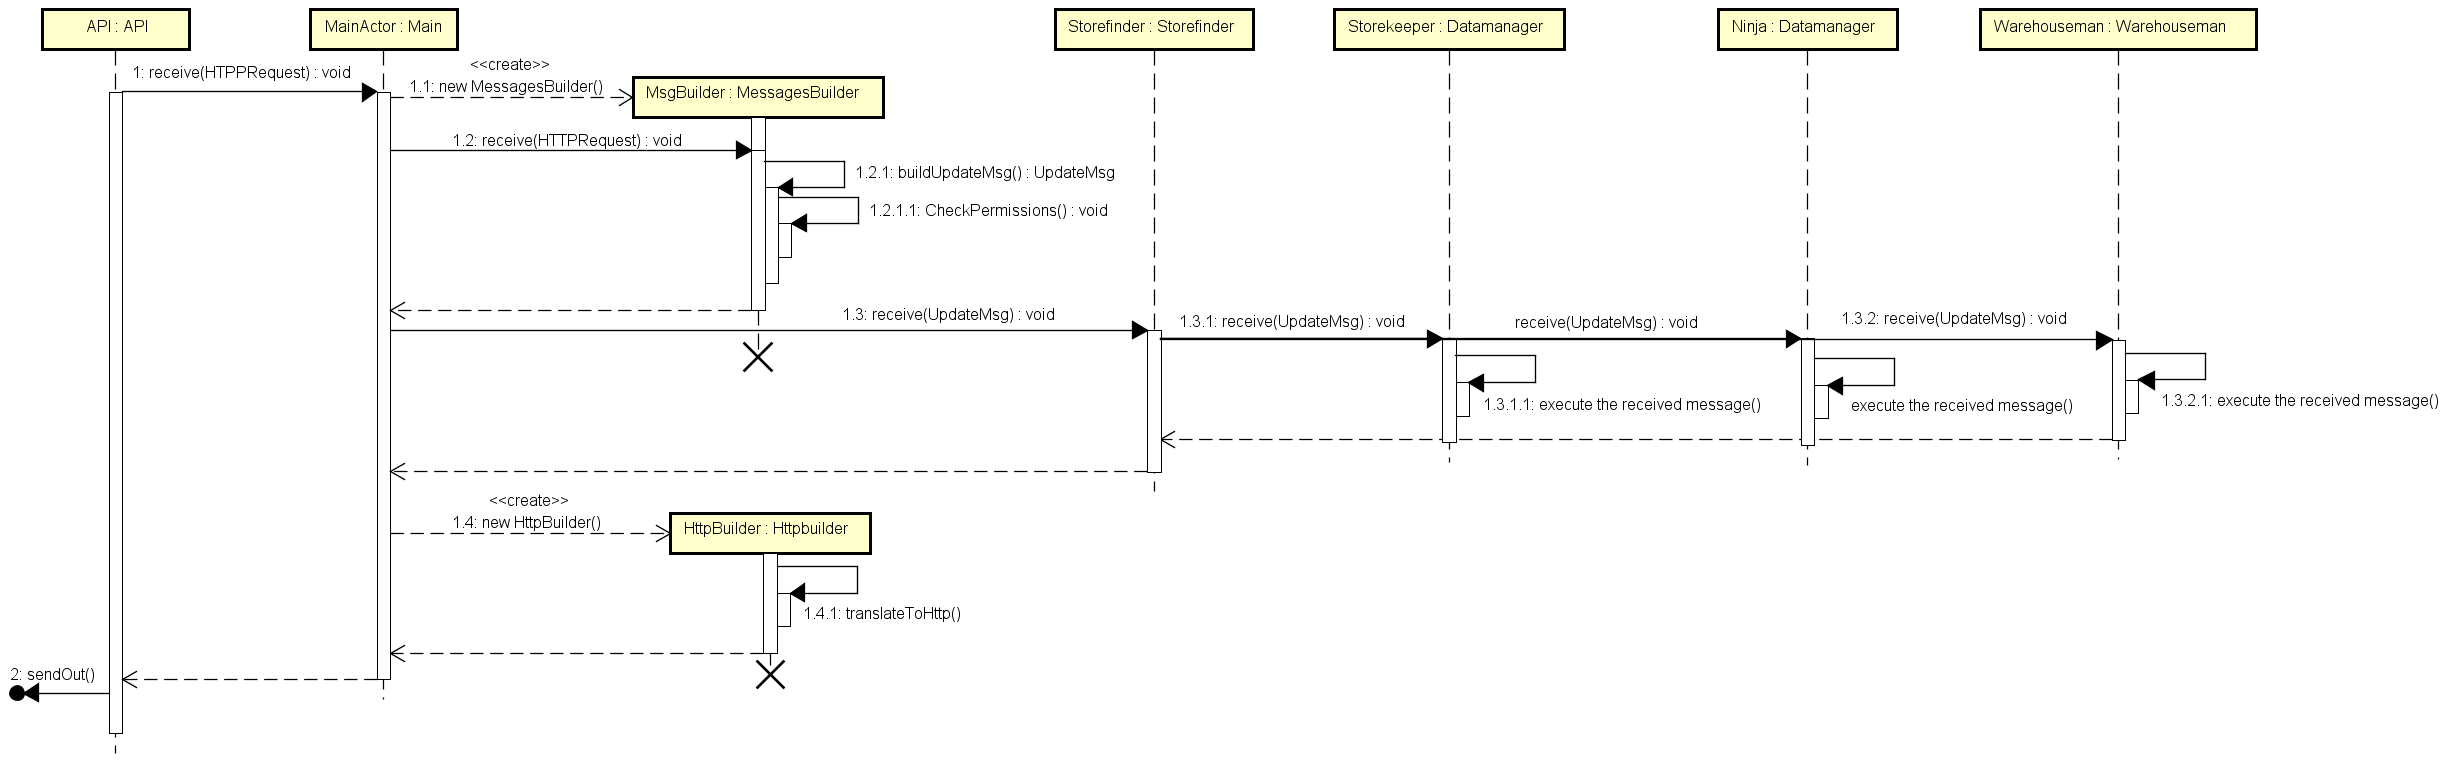
\includegraphics[width=\textwidth]{ST/seq/GestioneUpdateEntry.png}
				\caption{Diagramma di sequenza - gestione di richiesta di aggiornamento item.}
			\end{figure}
            Nel diagramma precedente è possibile visualizzare quali sono le operazioni che vengono eseguite per gestire una richiesta di aggiornamento di un item 
            all'interno di una mappa. La richiesta, arrivata allo Storekeeper come nel caso precedentemente visto, viene gestita in locale (la mappa viene aggiornata).
            Inoltre, in questo caso, l'attore Storefinder inoltra in messaggio di aggiornamento anche agli attori Ninja e Warehouseman corrispondendi allo Storekeeper 
            corretto. L'attore Ninja aggiorna come lo Storekeeper la sua mappa interna, mentre l'attore Warehouseman si occupa di aggiornare l'item su disco, in modo 
            da garantire persistenza dei dati. La risposta torna allo Storefinder, poi all'attore Main che come nei casi precedenti lo fa trasformare in HTTP e lo 
            inoltra all'esterno tramite API.
            
        \subsection{Creazione Ninja}
            \begin{figure} [H]
				\centering
				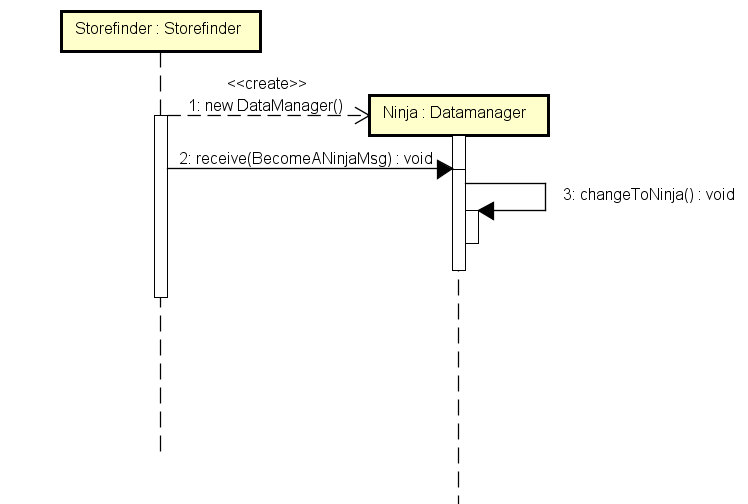
\includegraphics[width=\textwidth]{ST/seq/CreazioneNinja.png}
				\caption{Diagramma di sequenza - creazione di un attore Ninja.}
			\end{figure}
            Nel diagramma precedente è possibile visualizzare quali sono le operazioni che vengono eseguite per la creazione di un attore di tipo Ninja. 
            L'attore Storefinder crea un attore di tipo Datamanger, e immediatamente dopo gli invia un messaggio dedito alla sua trasformazione. L'attore 
            Datamanager non fa altro che chiamare un suo metodo, che tramite il metodo \textit{become()} fornito dalla libreria \textit{Akka} permette di 
            cambiare il comportamento di un attore alla ricezione di un messaggio.
         
         \subsection{Creazione Storekeeper}
            \begin{figure} [H]
				\centering
				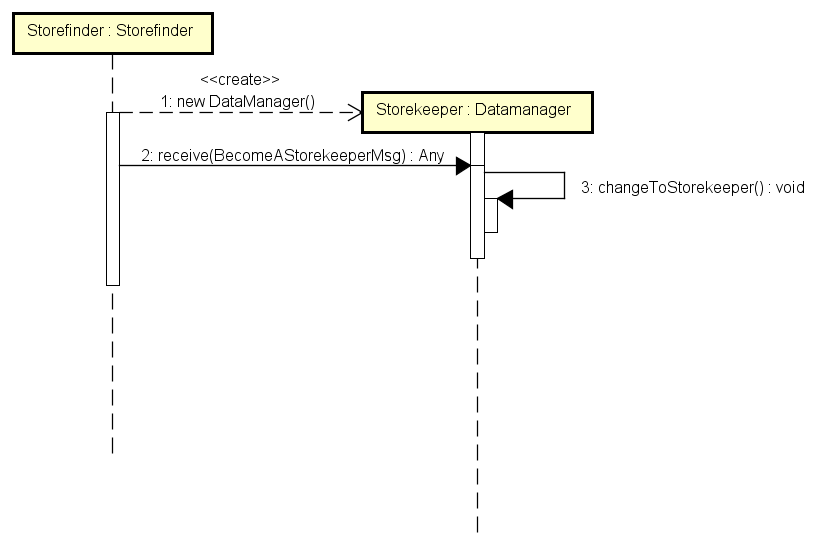
\includegraphics[width=\textwidth]{ST/seq/CreazioneStorekeeper.png}
				\caption{Diagramma di sequenza - creazione di un attore Storekeeper.}
			\end{figure}
            Nel diagramma precedente è possibile visualizzare quali sono le operazioni che vengono eseguite per la creazione di un attore di tipo Storekeeper.
            L'attore Storefinder crea un attore di tipo Datamanger, e immadiatamente dopo gli invia un messaggio dedito alla sua trasformazione. L'attore 
            Datamanager, come per il caso precedente, tramite il metodo \textit{become()} cambia il suo comportamento.
            
         \subsection{Sostituzione di uno Storekeeper}
            \begin{figure} [H]
				\centering
				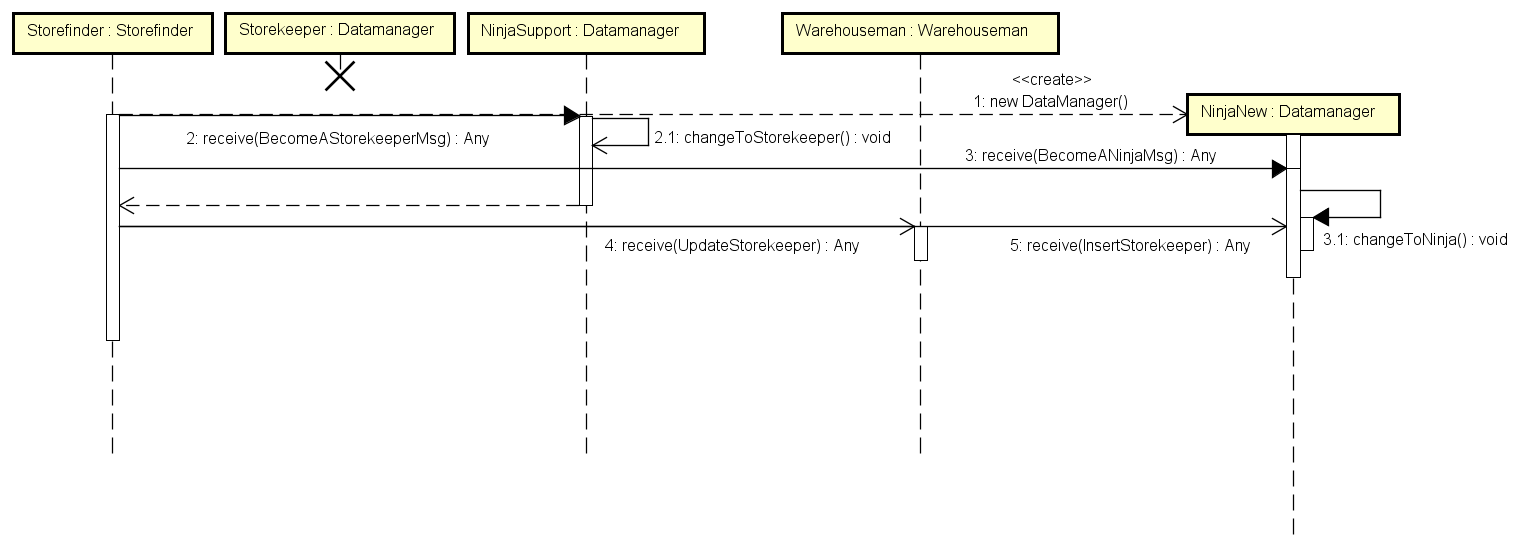
\includegraphics[width=\textwidth]{ST/seq/SostituzioneStorekeeper.png}
				\caption{Diagramma di sequenza - sostituzione di un attore Storekeeper.}
			\end{figure}
            Nel diagramma precedente è possibile visualizzare quali sono le operazioni che vengono eseguite quando è necessario sostiuire uno Storekeeper che 
            si è arrestato in modo anomalo. L'attore Storefinder manda un messaggio al Ninja di supporto dello Storekeeper morto in modo da fargli prendere il 
            suo posto. Successivamente crea un nuovo attore Ninja (come spiegato nel diagramma di sequenza visto prima) e notifica gli attori già esistenti del 
            cambio avvenuto.
            
        \subsection{Sequenza di un comando in client e driver}
            \begin{figure} [H]
                \centering
                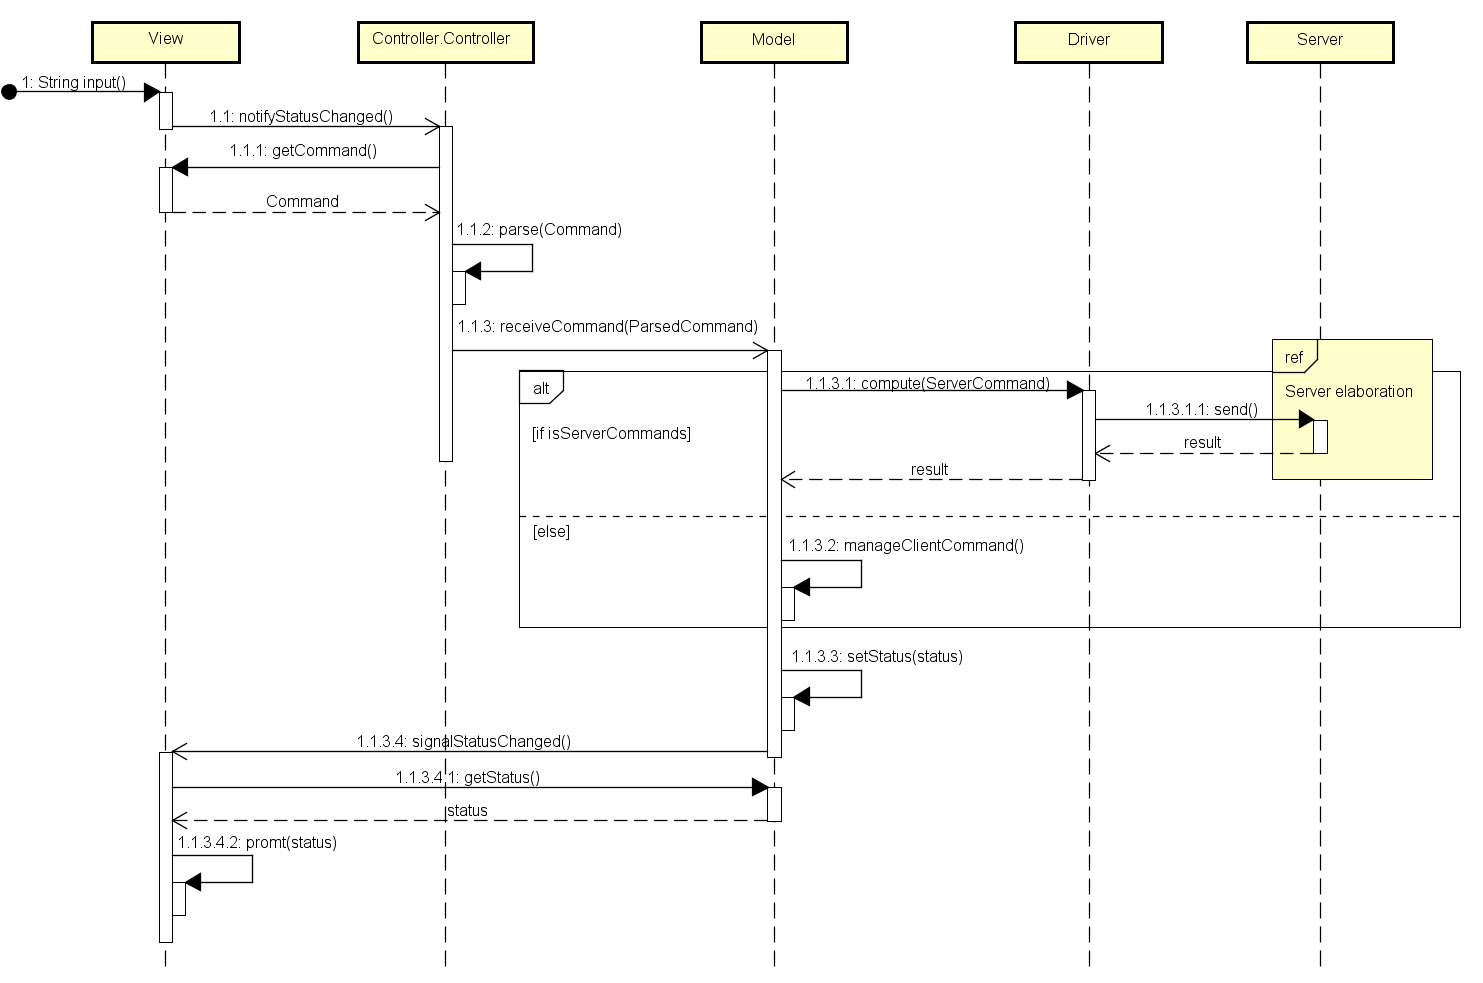
\includegraphics[width=\textwidth]{ST/seq/sequenzaClient.png}
                \caption{Diagramma di sequenza - sequenza di un comando in client e driver.}
            \end{figure}
            Nel diagramma precedente è possibile visualizzare quali sono le operazioni che vengono eseguite quando viene inserito un comando nella shell del client e viene premuto invio. \\
            La view notifica che il suo stato è cambiato e il controller prende la stringa inserita dall'utente per tradurla in un comando. Successivamente manda il comando al model. \\
            A questo punto la sequenza prevede due diversi flussi: se il comando riguarda il server viene inviato al driver che a sua volta lo invia al server per l'elaborazione. Quando il driver riceve una risposta, la ritorna al model del client che era rimasto in attesa. Se invece il comando non riguarda il server, come ad esempio il comando \texttt{HELP}, il model lo elabora al suo interno. In entrambi i casi alla fine viene generato ed impostato un nuovo stato del model e notificato il cambiamento. La  view quindi prende il nuovo stato e aggiorna il proprio di conseguenza, rendendolo visibile sulla shell per l'utente.

	\newpage 
	\section{Stime di fattibilità e di bisogno di risorse}
	
		L'architettura definita fino a questo punto è sufficiente per fornire una stima della fattibilità del prodotto e delle risorse richieste per la realizzazione. \\
	Il gruppo inizialmente non aveva conoscenze sufficienti per stimare in modo appropriato la complessità dell'implementazione di un Database basato sulla logica ad attori. Grazie al livello di dettaglio raggiunto sono stati fugati molti dei dubbi e delle incertezze a riguardo, confermando le previsioni sull'esito positivo del progetto. \\
	Sono state inoltre individuate con chiarezza le risorse tecnologiche che verranno utilizzate:
	\begin{itemize}
		\item Akka: libreria per modello ad attori.
		\item IntelliJ: framework per la stesura del codice.
		\item JVM: piattaforma per il funzionamento di Scala.
	\end{itemize}
	Il gruppo in contemporanea si è dedicato allo studio delle nuove tecnologie raggiungendo un buon livello di conoscenza. L'insieme di queste risorse potrà garantire la realizzazione di tutte le componenti dell'architettura.
	
	\newpage 
	\section{Tracciamento}
		\subsection{Tracciamento componenti-requisiti}
			\LTXtable{\textwidth}{tabelle_componenti_requisiti/componenti_requisiti.tex}
		\subsection{Tracciamento requisiti-componenti}
		
	\newpage 
	\section{Appendice}
	\subsection{Descrizione Design Pattern}
	Segue, per ogni Design Pattern utilizzato, la descrizione dello scopo, motivazione e applicabilità.
	\subsubsection{Event-driven}
				\begin{figure}[H]
					\centering
					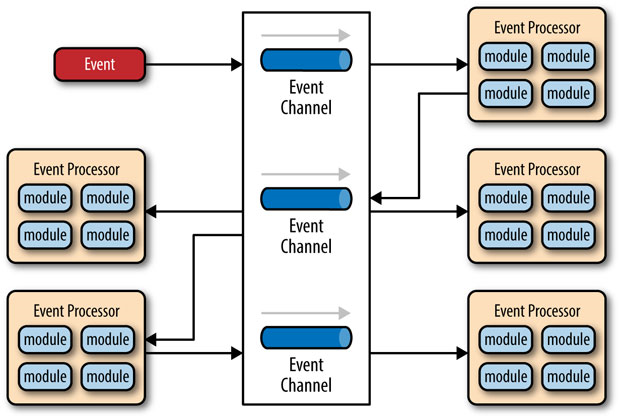
\includegraphics[scale=0.65]{immagini/ST/schemaevent-driven.png}
					\caption{Diagramma del Design Pattern Event-driven}
				\end{figure}
            \begin{itemize}
				\item \textbf{Scopo:}
					Produrre applicazioni molto scalabili e processare eventi asincroni disaccoppiati.
                \item \textbf{Motivazione:} Gestire le richieste che vengono volte all' applicativo tramite eventi processati in modo asincrono.
                \item \textbf{Applicabilità:}
                	Gestione di eventi attraverso l'utilizzo di un mediatore e elaboratori di eventi		
			\end{itemize}
	\subsubsection{MVC}
				\begin{figure}[H]
					\centering
					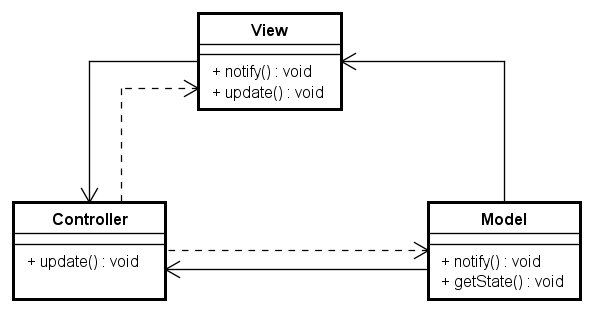
\includegraphics[scale=0.65]{immagini/ST/schemaMVC.png}
					\caption{Diagramma del Design Pattern MVC}
				\end{figure}
            \begin{itemize}
				\item \textbf{Scopo:}
					Disaccoppiamento delle seguenti componenti:
					\begin{itemize}
						\item Model regole di accesso e dati di business
						\item View rappresentazione grafica
						\item Controller reazioni della UI agli input utente
					\end{itemize}
                \item \textbf{Motivazione:}
                	Lo scopo di molti applicativi è di recuperare dati e mostrarli all'Utente. Si è visto che la migliore soluzione di questo scopo è dividere la modellazione del dominio, la presentazione e le reazioni basate sugli input degli utenti i tre classi separate, esistono vari design pattern che svolgono questa separazione, uno di questi è MVC; 
                \item \textbf{Applicabilità:}
					\begin{itemize}
						\item Applicazioni che devono presentare attraverso una UI un insieme di informazioni
						\item Le persone responsabili dello sviluppo hanno compentenze differenti
					\end{itemize}
                	 		
			\end{itemize}
	\subsubsection{Command}
				\begin{figure}[H]
					\centering
					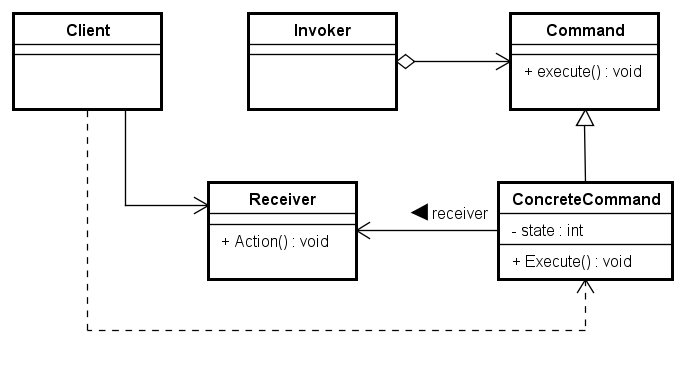
\includegraphics[scale=0.65]{immagini/ST/schemaCommand.png}
					\caption{Diagramma del Design Pattern Command}
				\end{figure}
            \begin{itemize}
				\item \textbf{Scopo:} Incapsulare una richiesta in un oggetto, cosicché i client siano indipendenti dalle richieste 
                \item \textbf{Motivazione:} Risolvere la necessità di gestire richieste di sui non si conoscono i particolari, tramite una classe astratta, Command, che definisce un interfaccia per eseguire la richiesta
                \item \textbf{Applicabilità:}
					\begin{itemize}
						\item Parametrizzazione di oggetti sull'azione da eseguire
						\item Specificare, accordare ed eseguire richieste molteplici volte
						\item Supporto ad operazioni di Undo e Redo
						\item Supporto a transazione, un comando equivale ad una operazione atomica
					\end{itemize}		
			\end{itemize}
				
	\subsubsection{Singleton}
				\begin{figure}[H]
					\centering
					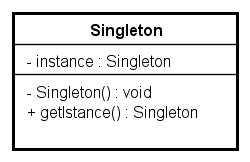
\includegraphics[scale=0.65]{immagini/ST/schemaSingleton.png}
					\caption{Diagramma del Design Pattern Command}
				\end{figure}
		\begin{itemize}
			\item \textbf{Scopo:} Assicurare che una classe abbia una sola istanza con un unico punto di accesso globale.
			\item \textbf{Motivazione:} È necessario assicurare che esista una sola istanza di alcune classi. Una classe Singleton ha la responsabilità sulle proprie istanze, in modo che nessuna altra istanza possa essere creata, e fornisce un punto di accesso unico.
			\item \textbf{Applicabilità:}
			\begin{itemize}
				\item Deve esistere una ed una sola istanza di una classe in tutta l'applicazione, accessibile dai client in modo noto.
				\item L'istanza deve essere estendibile con ereditarietà, consentendo ai client di non modificare il proprio codice.
			\end{itemize}
		\end{itemize}
	
	\cleardoublepage
	\addcontentsline{toc}{section}{\listfigurename}
	\listoffigures
	
	\cleardoublepage
	\addcontentsline{toc}{section}{\listtablename}
	\listoftables
		
\end{document}